\documentclass[../../几何与拓扑.tex]{subfiles}

\begin{document}
    

\chapter{基本群}

\section{同伦}

\begin{definition}
    设 \(  X,Y  \)是两个拓扑空间,\(  f,g  : X\to Y\)是两个连续映射.
    称 \(  f  \)同伦于 \(  g  \),记作 \(  \left( f\simeq g \right)   \),若
    存在连续映射 \(  F:X\times I\to Y  \),使得 \(  F\left(x,0 \right)= f\left( x \right)    \), \(  f\left( x,1 \right)= g\left( x \right)    \)对于所有的
     \(  x \in X  \)成立.   此时称映射 \(  F  \)为 \(  f  \)到 \(  g  \)的同伦.         
\end{definition}

\begin{remark}
    
    \begin{enumerate}
        \item 对于每个 \(  t \in I  \), \(  i _{t}: X \to X \times I\), \(  i _{t}\left( x \right) =  \left( x,t\right)    \)   是嵌入映射.故 \(  f_{t} =  F\circ i_{t}:X\to Y \)是从\(  X  \)到 \(  Y  \)的一组连续映射.
        \item \(  f_{0}= f,f_{1}= g  \).    
        \item 观察图\ref{graph:homotopy},每个 \(  t \in I  \)对应左侧一片圆, \(  t  \)比较近的圆映到 \(  Y  \)的图像是差不多的.   
    \end{enumerate}
    
\end{remark}
\begin{figure}[h]
    \centering
    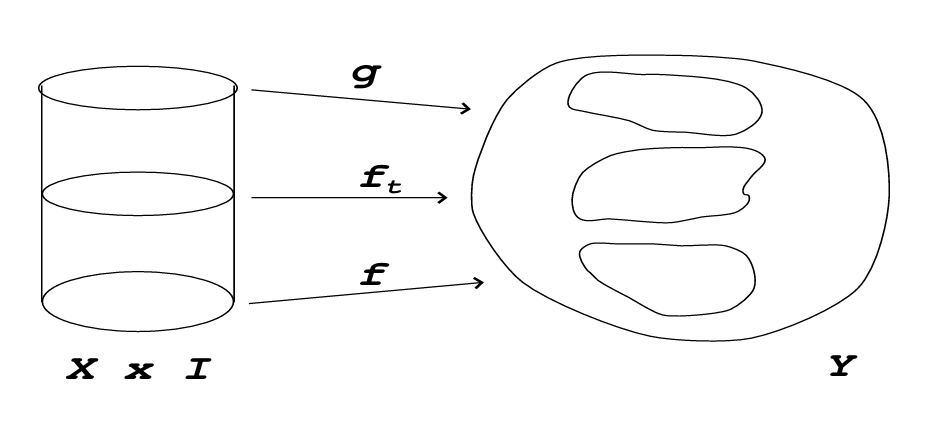
\includegraphics[scale=0.5]{homotopy.png}
    \caption{从  \(  f  \)到 \(  g  \)的同伦  }
    \label{graph:homotopy}
\end{figure}



\begin{example}
    设 \(  X  \)是拓扑空间, \(  Y  \)是 \(  \mathbb{R} ^{n}  \)上的凸集.令 \(  f,g:X\to Y  \)    是连续映射
    .则 \(  f  \)同伦于 \(  g  \).具体地, \(  H: X\times I\to Y  \) \[
    H\left( x,t \right) =  tg\left( x \right)+ \left( 1-t \right)f\left( x \right)    
    \]是 \(  f  \)到 \(  g  \)的同伦.此类同伦被称为是\textbf{直线同伦}.
\end{example}
\hspace*{\fill} 



\begin{example}
    设 \(  \mathbb{S}^{1} =  \left\{ z \in C : \left| z  \right|=  1  \right\}  \)是单位元.也可以写作 \(  \mathbb{S}^{1} =  \left\{ e^{i \theta }: 0\le  \theta \le 2\pi  \right\}  \).
    定义两个映射 \(  f,g  : \mathbb{S}^{1}\to \mathbb{S}^{1}\)   ,\(  f\left( z \right)= z,\text{和} g\left( z \right)= -z,z \in \mathbb{S}^{1}    \). 
    则 \(  f  \)同伦于 \(  g  \).具体地,定义 \(  F: \mathbb{S}^{1}\times I\to \mathbb{S}^{1}  \) \[
    F\left( e^{i \theta },t \right)=  e^{i\left(  \theta + t\pi  \right) } 
    \] 注意到 \(  F  \)是连续映射的复合 \[
    \begin{aligned}
    \mathbb{S}^{1}\times I \to \mathbb{S}^{1}\times \mathbb{S}^{1} \to \mathbb{S}^{1} \\ 
     \left( e^{i \theta },t \right) \to \left( e^{i \theta },e^{it\pi } \right)\to e^{i\left(  \theta + t\pi  \right) }  
    \end{aligned}
    \]其中第二个映射是复数的乘法,故 \(  F  \)是连续映射.此外,注意到映射族 \(  \left\{ f_{t}: \mathbb{S}^{1}\to \mathbb{S}^{1} \right\}  \)是旋转 \(  t\pi   ,0\le t\le 1\)的一族映射.        
\end{example}

\begin{theorem}
    设 \(  X,Y  \)是拓扑空间, \(  C\left( X,Y \right)   \)表示 \(  X  \)到 \(  Y  \)的全体连续映射.则同伦关系是 \(  C\left( X,Y \right)   \)
    上的一个等价关系.     
\end{theorem}

\begin{proof}

    对于连续映射 \(  f:X\to Y  \), 定义 \(  H\left( x,t \right)= f\left( x \right)    \)可以说明自反性.
    
    对于 \(  H: f\simeq g  \),定义 \(  H^{\prime} \left( x,t \right)= H\left( x,\left( 1-t \right)  \right)    \),则 \(  H^{\prime} :g\simeq f  \)  ,说明了对称性.

    对于 \(  H_1: f \simeq g,H_2:g\simeq h  \),定义H \[
    H\left( x,t \right): =  \begin{cases} H_1\left( x,2t \right),& 0\le t\le \frac{1}{2},\\ 
     H_2\left( x,2t-1 \right),& \frac{1}{2}\le t\le 1   \end{cases}  
    \]则由粘合引理 \(  H  \)是连续映射,说明了传递性.  

    \hfill $\square$
\end{proof}

\begin{definition}
    \(  C\left( X,Y \right)   \)上关于同伦关系的一个等价类,称为是一个同伦类. 同伦类的全体记作 \(  [X,Y]  \).  
\end{definition}

\begin{theorem}\label{同伦保复合}
    设 \(  f_1,g_1:X\to Y  \)是同伦的, 且\(  f_2,g_2:Y\to Z  \)是同伦的.则复合映射 \(  f_2\circ f_1,g_2\circ g_1: X\to Z  \)也是同伦的.   
\end{theorem}
\begin{proof}

    设 \(  H_1: f_1\simeq g_1  \), \(  H_2:f_2\simeq g_2  \).则 \(  f_2\circ H_1:X\times I\to Z  \)是 \(  f_2\circ f_1  \)到 \(  f_2\circ g_1  \)的同伦.
    接下来,定义 \(  H:X\times I\to Z  \), \(  H\left( x,t \right)= H_2\left( g_1\left( x \right)  ,t\right)    \).则 \(  H  \)是连续映射,且 \(  H\left( x,0 \right)= H_2\left( g_1\left( x \right),0  \right)= f_2\circ g_1\left( x \right)     \)         ,
     \(  H\left( x,1 \right) =  H_2\left( g_1\left( x \right),1  \right)= g_2\circ g_1\left( x \right)     \).现在 \(  f_2\circ f_1\simeq f_2\circ g_1, f_2\circ g_1\simeq g_2\circ g_1  \),因此 \(  f_2\circ f_1 \simeq  g_2\circ g_1  \).


    \hfill $\square$
\end{proof}

\hspace*{\fill}




\section{同伦型和可缩空间}


对于常值映射 \(  f:X \to Y  \),\(  f \equiv y_0  \),记它为 \(  C_{y_0}  \).


\begin{definition}{可缩}
    称拓扑空间 \(  X  \)是\textbf{可缩的},若单位映射 \(  I _{X}:X\to X  \)同伦于某个常值映射 \(  C_{x}:X \to X  \).称 \(  I _{X}  \)到 \(  C_{x}  \)  的同伦为空间到点 \(  x \in X  \)的一个\textbf{收缩}. 
\end{definition}

\begin{example}
     \(  \mathbb{R} ^{n}  \)上的凸集 \(  S  \)可以收缩到任意点 \(  x_0 \in S  \).   
\end{example}

\begin{definition}{星形集}
    称 \(  \mathbb{R} ^{n}  \)的子集 \(  X  \)是星形的,若存在 \(  x_0 \in X  \),使得任意点到 \(  x_0  \)的线段都落在 \(  X  \)上.   
\end{definition}

\begin{definition}{同伦等价,同伦型}
    设 \(  f:X \to Y  \)是连续映射.称 \(  f  \)是一个\textbf{同伦等价},若存在连续映射 \(  g:Y \to X  \),使得 \(  g\circ f  \)同伦于 \(  X  \)上的单位映射 \(  \operatorname{Id}_{X}  \),且 \(  f\circ g  \)同伦于 \(  Y  \)上的单位映射 \(  \operatorname{Id}_{_{Y}}  \).
    
    称两个拓扑空间 \(  X,Y  \)是\textbf{同伦等价的}或\textbf{有相同的同伦型},若存在其中一个空间到另一个空间的同伦等价. 
\end{definition}

\begin{remark}
    \begin{enumerate}
        \item 同胚的空间有相同的同伦型,在下面的例子中可以看到,有相同同伦型的空间不一定同胚.
    \end{enumerate}
    
\end{remark}


\begin{example}
    考虑单位(开或闭)圆盘 \(  \mathbb{D}^{2}  \),以及 \(  x_0 \in \mathbb{D}  \).令 \(  i: P =  \left\{ x_0 \right\}\to  \mathbb{D}^{2}  \)   是含入映射,
    \(  C_{x_0}:\mathbb{D}^{2}\to P  \)是常值映射.则 \(  C_{x_0}\circ i = \operatorname{Id}_{P}  \). 
    另一方面,考虑映射 \(  H: \mathbb{D}^{2}\times I \to \mathbb{D}^{2}  \), \[
    H\left( x,t \right) = \left( 1-t \right)x+ tx_0  
    \]   是 \(  \operatorname{Id}_{\mathbb{D}^{2}}  \)到 \(  i\circ C_{x_0}  \)  的同伦.因此 \(  \mathbb{D}^{2}  \)与点空间 \(  P  \)有相同的同伦型,而它们显然是不同胚的.  

\end{example}

\begin{remark}
   \begin{enumerate}
    \item  也可以看到紧致性并非同伦不变的.
    \item 类似地,很多拓扑不变量都不是同伦不变的,可见同伦分类是一种比较弱的分类.
   \end{enumerate}
   
\end{remark}

\hspace*{\fill} 


接下来给出一些同伦不变量,那么它们显然也是拓扑不变的.一但我们发现两个拓扑空间的某个同伦不变量是不同的,
则它们是不同伦的,进而不是同胚的,这给出判断两个空间不同胚的方式.





\begin{theorem}
    一个拓扑空间 \(  X  \)是可缩的,当且仅当 \(  X  \)与一个点空间 \(  P =  \left\{ p \right\}  \)具有相同的同伦型.   
\end{theorem}

\begin{proof}

    设拓扑空间 \(  X  \)是可缩的,设 \(  H:X \times I\to X\)是 \(  \operatorname{Id}_{X}  \)   到常值映射 \(  C_{x_0}:X \to X  \)的同伦.定义 \(  i: P \to X  \),\(  i\left( p \right)= x_0   \),\(  C:X \to P  \), \(  C\left( x \right)= p   \).
    则 \(  i\circ C =  C_{x_0} \simeq  \operatorname{Id}_{X}  \), \(  C\circ i  = \operatorname{Id}_{P}  \).因此 \(  X  \)和 \(  P  \)有相同的同伦型.
    
    反之,若设 \(  X  \), \(  P  \)有相同的同伦型,则存在 \(  f:X \to P  \), \(  g:P\to X  \),使得 \(  f\circ g = \operatorname{Id}_{P}  \), \(  g\circ f \simeq \operatorname{Id}_{X}  \).设 \(  H: g \circ f \simeq  \operatorname{Id}_{X}  \). 设 \(  g\left( p \right)= x_0   \),又 \(  f\left( x \right)= p   \),故 \(  g\circ f \equiv x_0  \)是常值映射.  这表明 \(  X  \)是可缩的.        

    \hfill $\square$
\end{proof}

\begin{proposition}
    设 \(  X  \)是可缩空间,则 \(  X  \)是道路连通的.  
\end{proposition}

\begin{proof}

    设 \(  X  \)是可缩空间, \(  H: \operatorname{Id}_{X}\simeq  C_{x_0}  \).   
    
    任取 \(  x_1,x_2 \in X  \),则 \( f_{x_1}\left( t \right): =    H\left( x_1,t \right)   \) 和 \(  f_{x_2}\left( t \right): =  H\left( x_2,t \right)    \)是连续映射,使得 \(  f_{x_1}\left( 0 \right)= x_1,f_{x_1}\left( 1 \right)= x_0    \), \(  f_{x_2}\left( 0 \right)= x_2,f_{x_2}\left( 1 \right)= x_0    \).
    定义 \(  g\left( t \right)   \)  \[
    g\left( t \right): =  \begin{cases}  f_{x_1}\left( 2t \right),& t \in [0, \frac{1}{2}]\\ 
     f_{x_2}\left( 2-2t \right),& t \in [\frac{1}{2},1]   \end{cases}  
    \]则 \(  g\left( t \right)   \)是连续映射,使得 \(  g\left( 0 \right)=  x_1   \), \(  g\left( 1 \right)= x_2   \),这表明 \(  X  \)是道路连通的.    

    \hfill $\square$
\end{proof}



\begin{proposition}
    拓扑空间 \(  X  \)是可缩的,当且仅当任意拓扑空间 \(  T  \)到 \(  X  \)的任意映射 \(  f:T \to X  \)是同伦于常值映射的.    
\end{proposition}
\begin{remark}
    \begin{enumerate}
        \item 习题给出 \(  f: X\to T  \)的情况也成立. 
    \end{enumerate}
    
\end{remark}

\begin{proof}

    若 \(  X  \)是可缩的,存在\(  x_0 \in X  \),以及 \(  H: \operatorname{Id}_{X}\simeq  C_{x_0}  \).任取拓扑空间 \(  T  \)和映射 \(  f: T\to X  \),则由 定理 \ref{同伦保复合} , \(  f =  \operatorname{Id}_{X}\circ f  \simeq C_{x_0}\circ f\)是常值映射.
    
    
    反之,若任取拓扑空间 \(  X  \),以及映射 \(  f: T\to X  \),都有 \(  f  \)同伦于常值映射,特别地取 \(  T =  X  \), \(  f= \operatorname{Id}_{X}  \),则 \(  \operatorname{Id}_{X}\simeq  C_{x_0}  \)对某个 \(  x_0 \in X  \)成立,故 \(  X  \)是可缩的       .   

    \hfill $\square$
\end{proof}


\begin{corollary}
    设 \(  X  \)是可缩空间,则单位映射 \(  \operatorname{Id}_{X}: X\to X  \)  同伦于常值映射 \(  C_{x}: X\to X  \)  对于任意的 \(  x \in X  \)成立.特别地, \(  X  \)可以收缩到 \(  X  \)上的任意一点.      
\end{corollary}

\begin{proof}

    设 \(  X  \)是可缩空间, 上面命题的证明表示,若 \(  \operatorname{Id}_{X}\simeq  C_{x_0}: X \to X  \) ,则任意映射 \(  f: T\to X  \)都可以同伦到一个恒为 \(  x_0  \)的常值映射.特别地取 \(  T =  X  \), \(  f =  C_{x}: X \to X  \),则 \(  C_{x}\simeq  C_{x_0}  \simeq  \operatorname{Id}_{X}\)  .    

    \hfill $\square$
\end{proof}

\begin{definition}{相对同伦}
    令 \(  A\subseteq X  \)是任意子集,\(  f,g;X \to Y  \)是两个连续映射.称 \(  f  \)是相对 \(  A  \)同伦于 \(  g  \)的,若存在连续映射\(  F  :X\times I\to Y\),使得  \[
    F\left( x,0 \right)= f\left( x \right),F\left( x,1 \right)= g\left( x \right),\forall x \in X    
    \],并且 \[
    F\left( a,t \right)= f\left( a \right)= g\left( a \right),\forall    a \in A   
    \]      
\end{definition}

\begin{remark}
    \begin{enumerate}
        \item 如果令 \(  A   =  \varnothing\),就得到了同伦的概念.
        \item 特别地,如果 \(  f,g  \)相对于 \(  A  \)同伦,则在一开始时它们就在 \(  A  \)上一致.
        \item \(  f  \)相对于 \(  A  \)同伦于 \(  g  \)是说, \(  f  \)可以通过一族在 \(  A  \)上保持相同的连续映射变动到 \(  g  \).
        \item 不难证明相对于 \(  A  \)同伦是 \(  C\left( X,Y \right)   \)上的一个等价关系.            
    \end{enumerate}
    
\end{remark}


\begin{theorem}
    若 \(  X  \)是相对于 \(  \left\{ a \right\}  \) 可缩到点 \(  a \in X  \)的空间 .则对于 \(  a  \)在 \(  X  \)中的任意邻域 \(  U  \),存在 \(  a  \)含于 \(  U  \)的一个邻域 \(  V  \),
    使得 \(  V  \)上的任意一点都可以通过一个落在 \(  U  \)上的道路连接到 \(  a  \),即 \(  X  \)是\textbf{半-局部道路连通}的.           
\end{theorem}

\begin{note}

    \begin{enumerate}
        \item 要求收缩是相对于 \(  \left\{ a \right\}  \)的,保证了对于任意的 \(  t \in I  \),都有 \(  F\left( a,t \right) \in U   \),从而可以找到 \(  a,t  \)的邻域使得像含于 \(  U  \).     
    \end{enumerate}
    

\end{note}
\begin{proof}

    若 \(  X  \)满足条件,则 存在连续映射 \(  F: X\times I\to  X  \),使得 \(  F\left( x,1 \right)= a,\forall  x \in X   \),且 \(  F\left( a,t \right)= a, \forall  t \in I   \).
    
   由 \(  F  \)连续性,对于任意的 \(  t \in I  \),存在 \(  a,t  \)的开邻域 \(  V_{t}\left( a \right)   \)和 \(  W\left( t \right)   \),使得 \(  F\left( V_{t}\left( a \right)\times W\left( t \right)   \right)\subseteq U   \).\(  \left\{ W\left( t \right)  \right\}_{t \in I}  \)构成 \(  I  \)的一个开覆盖,由 \(  I  \)的紧性,存在有限的子覆盖
    \(  W\left( t_1 \right),\cdots ,W\left( t_{n} \right)    \)         .

    现在 令\(V\left( a \right): =     \bigcap_{i}V_{t_{i}}  \left( a \right)  \)是 \(  a  \)的一个开邻域,则 \(  F\left( V\left( a \right) \times  \bigcup_{i} W\left( t_{i} \right)   \right)  =  F\left( V\left( a \right)\times I  \right) \subseteq U   \).
    任取  \(  i =   1,\cdots,n   \)和 \(  x \in  V_{t_{i}}\left( a \right)   \),         
    由于 \(  F\left( x,1 \right)= a   \),\(  F\left( x,0 \right)= x   \),因此 \(  t\mapsto F\left( x,t \right), t \in I   \)使得落在 \(  U  \)的连接 \(  x  \)和 \(  a  \)的道路.     
    \hfill $\square$
\end{proof}

\begin{example}(Comb Space)
    考虑以下集合 \(  C  \) ,它由从 \(  \left( 0,0 \right)   \)到 \(  \left( 0,1 \right)   \)的水平线段和所有 \(  \left( \frac{1}{n},0 \right)   \)到 \(  \left( \frac{1}{n},1 \right)   \)的垂直线段组成,其中 \(  n =  1,2,\cdots   \).     

    \begin{enumerate}
        \item \textbf{\(  C  \)是可缩的  }.投影映射 \(  p: C\to L  \)是同伦等价,其中 \(  L  \)是水平线 ,事实上, 
         \(  i: L \to C  \)是含入映射,则 \(  p\circ i =   \operatorname{Id}_{L} \).另一方面,定义 \(  F: C\times  I \to C  \), \[
         F\left( \left( x,y \right),t  \right) : =  \left( x,\left( 1-t \right)y  \right)   
         \],则 \(  F :\operatorname{Id}_{L}\simeq i\circ p  \).而 \(  L  \)同胚由单位开区间是可缩的,又 \(  C  \)于 \(  L  \)有相同的同伦型,  因此 \(  C  \)是可缩的. 
        \item \(  C  \)不是相对于 \(  \left\{ \left( 0,1 \right)  \right\}  \)可缩的.取 \(  \left( 0,1 \right)   \)的半径为 \(  \frac{1}{2}  \)的圆盘邻域 \( D  \) ,
        则任意含于\(  D  \) 的邻域上,都有无穷多个连通分支,由上面的定理可知, \(  C  \)不是相对于 \(  \left\{ \left( 0,1 \right)  \right\}  \)可缩的.    
    \end{enumerate}
    
\end{example}


\hspace*{\fill} 


\begin{definition}
    令 \(  A\subseteq X  \).称 \(  A  \)是 \(  X  \)的一个\textbf{收缩},若存在连续映射 \(  r: X\to A  \),使得 \(  r\left( a \right)= a,\forall  a \in A   \).此时称映射 \(  r  \)为\textbf{收缩映射}.      
\end{definition}

\begin{remark}
    \begin{enumerate}
        \item  \(  A  \)是 \(  X  \)的一个收缩,当且仅当含入映射 \(  i: A \to X  \)有连续的左逆.
        \item 易见此时 \(  A  \)的子空间也是 \(  X  \)的一个收缩.   
        \item 任意拓扑空间 \(  X  \)上的每个点 \(  x_0 \in X  \)都是 \(  X  \)的一个收缩,收缩映射为 \(  C_{x_0}  \).
        \item 当 \(  A  \)是 \(  X  \)的收缩时,  若 \(  X  \)连通,则 \(  A  \)亦然.            
    \end{enumerate}
    
\end{remark}

\begin{definition}
    称拓扑空间 \(  X  \)是可以形变到子空间 \(  A \subseteq X  \)的,若存在含入映射 \(  i: A \to X  \)的同伦右逆 \(  f: X \to A  \),即单位映射 \(  \operatorname{Id}_{X}  \)同伦于 \(  i \circ f: X \to X  \).       
\end{definition}

\begin{remark}
    \begin{enumerate}
        \item 也就是说,存在同伦 \(  D: X \times I \to X  \),使得 \[
        D\left( x,0 \right)= x, D\left( x,1 \right)= i\left( f\left( x \right)  \right)= f\left( x \right)    
        \] 
        \item 称这样的同伦 \(  D  \)为 \(  X  \)到 \(  A  \)的一个形变.
        \item 直观地讲,存在一个连续的形变 \(  D  \), 将\(  X  \)上每一个点连续变形到 \(  A  \)中的点.    
        \item 特别地,取 \(  A =  \left\{ a \right\}  \), \(  a \in X  \),就得到可缩的概念.
    \end{enumerate}
    
\end{remark}


\begin{definition}
    称拓扑空间 \(  X  \)是可以 \textbf{强形变}到子空间 \(  A  \)的,若含入映射 \(  i : A \to X  \)有相对于 \(  A  \)的连续同伦右逆,即单位映射 \(  I _{X}: X \to X  \)相对于 \(  A  \)同伦于 \(  i\circ f : X \to X  \)        
\end{definition}

\begin{remark}
\begin{enumerate}
    \item 设 \(  D  \)是 \(  \operatorname{Id}_{X}  \)相对于 \(  A  \)到 \(  i\circ f  \)的同伦.则 \(  D\left( a,1 \right)= f\left( a \right)= a ,\forall  a \in A    \).此时 \(  f: X \to A  \)自动是 \(  X  \)到\(  A  \)的一个收缩. 即,强形变的终映射是一个收缩.
    \item 形变的终映射是收缩不一定导出形变是强形变.
\end{enumerate}

\end{remark}


\begin{definition}
    称拓扑空间 \(  X  \)的子空间 \(  A  \)是 \(  X  \)的一个\textbf{形变收缩},若 \(  X  \)可以形变到 \(  A  \),且形变的终映射是 \(  X  \)到 \(  A  \)的一个收缩.       
\end{definition}

\begin{remark}
    \begin{enumerate}
        \item 形变收缩较强形变来说弱一点,强形变是说让 \(  X  \)上的点都能跑到 \(  A  \)里面,且一直保持 \(  A  \)中的点不动,形变收缩是指 \(  A  \)中的点中间可以来回跑,但是最后要回到自己的位置上.     
    \end{enumerate}
    
\end{remark}


为了做强调, 不妨也语意冗余地给出一个定义\footnote{即便强形变的终映射已经是一个收缩了}
\begin{definition}
    设 \(  X  \)是拓扑空间, \(  A  \)是 \(  X  \)的一个子空间.称 \(  A  \)是 \(  X  \)的一个\textbf{强形变收缩},若 \(  X  \)可以强形变到 \(  A  \),且形变的终映射是 \(  X  \)到 \(  A  \)的一个收缩.      
\end{definition}

\begin{remark}
    \begin{enumerate}
        \item 此时,含入映射 \(  i: A \to X  \)有双边的同伦逆,进而是同伦等价. 
    \end{enumerate}
    
\end{remark}

\begin{example}
    对于 \(  n\ge 1, \mathbb{S}^{n} \subseteq \mathbb{R} ^{n+ 1} - \left\{ \left( 0,\cdots ,0 \right)  \right\}= X  \)是 \(  X  \)的一个强形变收缩.         
\end{example}

\begin{proof}

        定义 \[
        D\left( x,t \right)= \left( 1-t \right)x +  t \frac{x }{\left\| x \right\| }   
        \]则 \( D: [\mathbb{R} ^{n+ 1}-\left\{ \left( 0,\cdots ,0 \right)  \right\}]\times I \to  [\mathbb{R} ^{n+ 1}-\left\{ \left( 0,\cdots ,0 \right)  \right\}]  \)是连续映射.
        始映射为 \(  \operatorname{Id}_{X}  \),终映射为 \(  x \mapsto \frac{x }{\left\| x \right\| }   \)为 \(  \mathbb{R} ^{n+ 1}-\left\{ \left( 0,\cdots ,0 \right)  \right\}  \)到 \(  \mathbb{S}^{n}  \)    的一个收缩.

    \hfill $\square$
\end{proof}

\hspace*{\fill} 

\section{基本群及其性质}

\begin{definition}{道路的等价}
    设 \(  X  \)是拓扑空间, \(   \alpha , \beta   \)是 \(  X  \)上的两条有相同端点的道路,即 \(   \alpha \left( 0 \right)=  \beta \left( 0 \right)= x_0    , \alpha \left( 1 \right)= \beta \left( 1 \right)= x_1  \) .
    称 \(  \alpha   \)和 \(  \beta   \)是等价的,记作 \(   \alpha \sim _{\left( x_0,x_1 \right) }\beta   \), 若存在他们之间的保端点的同伦,即存在相对于 \(  \alpha   \)和 \(  \beta   \)之间相对于 \(  \left\{ 0,1 \right\}  \subseteq I\)的同伦.        
\end{definition}

\begin{remark}
    \begin{enumerate}
        \item 通常称这样的一个同伦为道路同伦.
    \end{enumerate}
    
\end{remark}

\begin{theorem}
    设 \(  X  \)是拓扑空间 ,\(  x_0,x_1 \in X  \).则道路的等价确实给出 全体以 \(  x_0  \)为起点, \(  x_1  \)为终点的道路的一个等价关系.    
\end{theorem}

\begin{proof}

    令 \(   \alpha : I \to X  \)是道路,使得 \(  \alpha \left( 0 \right)= x_0   \), \(  \alpha \left( 1 \right)= x_1   \).定义 \(  H\left( s,t \right): =    \alpha \left( s \right)    \),则 \(  H  \) 是   \(  \alpha   \)到
    自身的相对于 \(  \left\{ 0,1 \right\}  \)的同伦,说明了自反性.
    
    接下来,设  \(  G  \)是 \(  \alpha   \)到 \(  \beta   \)的道路同伦.定义 \(  H\left( s,t \right)=  G\left( s,1-t \right)    \).则 \(  H  \)是 \(  \beta   \)到 \(  \alpha   \)的道路同伦,这就说明了传递性.
    
    最后,设 \(  H  \)是 \(  \alpha   \)到 \(  \beta   \)的道路同伦, \(  G  \)是 \(  \beta   \)到 \(  \gamma  \)的道路同伦,定义 \(  K:I \times I \to X  \), \[
    K=  \begin{cases} H\left( s,2t \right),& t \in [0,\frac{1}{2}]  \\ 
     G\left( s, 2t-1\right),& t \in [\frac{1}{2},1] \end{cases} 
    \]       则 \(  G  \)是 \(   \alpha   \)到 \(   \gamma   \)的道路同伦,这就说明了传递性  . 

    \hfill $\square$
\end{proof}


\begin{corollary}
  道路的等价也给出  \(  X  \)上所有以\(  x_0 \in X  \)为基点的循环  中的一个等价关系.
\end{corollary}


\begin{remark}
    \begin{enumerate}
        \item 以下记以 \(  x_0  \)为基点的循环 \(  \alpha   \)和 \(  \beta   \)等价,为 \(  \alpha \sim_{ x_0 }\beta   \).
        \item 记 \(  \alpha   \)所在的循环的道路等价类为 \(  [ \alpha ]  \),也称作循环 \(  \alpha   \)的同伦类.
        \item 令 \(  \pi _1 \left( X,x_0 \right)   \)表示 \(  X  \)上以 \(  x_0  \)为基点的循环的同伦类的全体.即 \[
        \pi \left( X,x_0 \right)= \left\{ [ \alpha ]:  \alpha \text{是}X \text{上以} x_0 \text{为基点的循环} \right\} 
        \]            
    \end{enumerate}
    
\end{remark}

\begin{proposition}
    设 \(   \alpha , \beta , \alpha ^{\prime} , \beta ^{\prime}   \)是 \(  X  \)上以 \(  x_0  \)为基点的循环,并且\(\alpha \sim _{x_0}  \alpha ^{\prime}  , \beta \sim _{x_0} \beta ^{\prime}   \)    
    ,则 \(  \alpha * \beta \sim _{x_0} \alpha ^{\prime} *\beta ^{\prime}   \) 
\end{proposition}

\begin{proof}

    设 \(  H_1,H_2  \)分别是  \(  \alpha   \)到 \(   \alpha ^{\prime}   \)和 \(  \beta   \)到 \(  \beta ^{\prime}   \)的同伦.
    
    定义 \(  H: I \times I \to X  \), \[
    H\left( s,t \right)=  \begin{cases} H_1\left( 2s,t \right),& s \in [0,\frac{1}{2}]\\ 
     H_2\left( 2s-1,t \right),& s \in [\frac{1}{2},1]   \end{cases}  
    \]则 \(  H\left( s,0 \right) =  \left( \alpha *\beta  \right)\left( s \right)     \)  , \(  H\left( s,1 \right)= \left(  \alpha ^{\prime} *\beta ^{\prime}  \right)\left( s \right)     \),并且 \(  H\left( 0,t \right)= x_0= H\left( 1,t \right)    \).因此 \(  \alpha *\beta \sim _{x_0}  \alpha ^{\prime} *  \beta ^{\prime}   \)   

    \hfill $\square$
\end{proof}


\begin{corollary}
    设 \(  \alpha   \)和 \(  \alpha ^{\prime}   \)是 \(  x_0  \)到 \(  x_1  \)的同伦的道路, \(  \beta   \)和 \(  \beta ^{\prime}   \)是
    \(  x_1  \)到 \(  x_2  \)的同伦的道路,则 \(  \alpha *\beta   \)和 \(   \alpha ^{\prime} *\beta ^{\prime}   \)是从 \(  x_0  \)到\(  x_2  \)的同伦的道路,并且同伦可以被选取为使得 \(  x_1  \)不变的.             
\end{corollary}
\begin{proof}

    仿照上个命题即可.

    \hfill $\square$
\end{proof}


\begin{definition}
    若 \(  \alpha   \)是从 \(  x_0  \)到 \(  x_1  \)的道路,则\(  [ \alpha ]  \)通常表示为 \(  \alpha   \)所在的 \(  x_0  \)到 \(  x_1  \)的道路同伦类.  
    
    拓扑空间 \(  X  \)上从 \(  x_0  \)到 \(  x_1  \)的全体道路同伦类记作 \(  \pi _1 \left( X,x_0,x_1 \right)   \).    
\end{definition}

\begin{definition}{乘法运算}
    定义 \(  \pi _1 \left( X,x_0,x_1 \right)   \)上的运算 \[
    \circ : \pi _1 \left( X,x_0,x_1 \right)\times \pi \left( X,x_1,x_2 \right)\to \pi _1 \left( X,x_0,x_2 \right)   
    \] 按以下方式 \[
    [ \alpha ]\circ [ \beta ]: =  [ \alpha *\beta ]
    \]
\end{definition}

\begin{remark}
    \begin{enumerate}
        \item 上面的推论给出了良定义性.
    \end{enumerate}
    
\end{remark}

\begin{theorem}
    \(  \pi _1 \left( X,x_0 \right)   \)在运算“\(  \circ  \)”构成群.  
\end{theorem}
\begin{remark}
    以下证明都可以稍作改变,给出在非循环的道路中对应性质的证明:
    \begin{enumerate}
        \item 设 \(  \alpha   \)是 \(  x_0  \)到 \(  x_1  \)的道路, \(  \beta   \)是 \(  x_1  \)到 \(  x_2  \)的道路, \(   \gamma   \)是 \(  x_2  \)到 \(  x_3  \)的道路,则 \[
        \left( [ \alpha ]\circ [\beta ] \right)\circ [ \gamma ] =  [ \alpha ]\circ \left( [\beta ]\circ [ \gamma ] \right)  
        \]         
        \item 设 \(  \alpha   \)是 \(  x_0  \)到 \(  x_1  \)的道路,那么 
        \begin{enumerate}
            \item \(  [C_{x_0}] \circ [ \alpha ]=  [C_{x_0}* \alpha ]= [ \alpha ]  \) 
            \item \(  [ \alpha ]\circ [C_{x_1}] = [ \alpha * C_{x_1}] = [ \alpha ]\) 
        \end{enumerate}
        \item 设 \(  \alpha   \)是 \(  x_0  \)到 \(  x_1  \)的道路,那么 
        \begin{enumerate}
            \item \(  [ \alpha ]\circ [ \alpha ^{-1} ] =  [C_{x_0}]  \)
            \item \(  [ \alpha ^{-1} ]\circ [ \alpha ]=  [C_{x_1}]  \)  
        \end{enumerate}
           
    \end{enumerate}
     
\end{remark}
\begin{proof}

    \textbf{结合律}:
    只需要说明 \(  \left( \alpha *\beta  \right)* \gamma \sim _{x_0} \alpha *\left( \beta * \gamma  \right)    \) 
    为此,定义 \(  H:X \times I \to  X  \), \[
    H\left( x,t \right): =  \begin{cases} \alpha \left( \frac{4s}{t+ 1} \right) ,& s \in [0, \frac{1}{4}\left( 1+ t \right) ]\\ 
      \beta \left( 4s-1-t \right),& s \in [ \frac{1}{4}\left( 1+ t \right) ,\frac{1}{4}\left( 2+ t \right) ]  \\ 
      \gamma \left( \frac{4s-2-t }{2-t }  \right),& s \in [\frac{1}{4}\left( 2+ t \right),1 ] \end{cases}  
    \] 即可.
    \begin{note}
    
        想法是随 \(  t  \)的变换改变道路的比例,因此分别改变 \(   \alpha , \beta , \gamma   \)的取值范围.
        
        先分别确定各道路在 \(  I _{s}  \)上分配到的两端点随时间的变化,再依变化调整道路括号内的数,对于后者可以通过线性函数 \(  f\left( x \right)=  \frac{f\left( b \right)-f\left( a \right)   }{b-a } \left( x-a \right)     \),取 \(  f\left( b \right)= 1   \), \(  f\left( a \right)= 0   \)     ,\(  a,b  \)分别是道路在 \(  I _{s}  \)上的两端点   来构造,
        例如对 \(  \alpha   \)就可以确定最后的一个分段为 \(  \alpha \circ f  \).  
    
    \end{note}

    \textbf{接下来说明单位元的存在性}:
    我们说明 \(  C_{x_0}  \)所在的等价类 \(  [C_{x_0}]  \) 是单位元.为此,只需要说明 \(   \alpha *C_{x_0} \sim _{x_0} \alpha   \)  以及 \(  C_{x_0} * \alpha \sim  _{x_0} \alpha  \).
    
    对于前者,定义 \(  H: X \times  I \to X  \) \[
    H\left( x,t \right) = \begin{cases}  \alpha \left( \frac{2s}{t+ 1} \right),& s \in [0,\frac{1}{2}\left( t+ 1 \right)  ]\\ 
    x_0,&  s \in  [\frac{1}{2}\left( t+ 1 \right),1 ] \end{cases}  
    \] 后者 是类似的.

    \textbf{最后说明 \(  \pi _1 \left( X,x_0 \right)   \)中任意元素皆可逆 }: 对于 \(  [ \alpha ] \in \pi _1 \left( X,x_0 \right)   \),定义 \(   \alpha ^{\prime} \left( t \right)=   \alpha \left( 1-t \right)    \),只需说明 \(  [ \alpha ^{\prime} ]  \)  与 \(  \alpha   \)的选取无关,并且 \(  [ \alpha ^{\prime} ]  \)是 \(  [ \alpha ]  \)的逆.
        对于第一个断言,设 \(  \beta \sim _{x_0}\alpha   \), \(  H  \)是对应的道路同伦.定义 \(  H^{\prime}   \) \[
        H^{\prime} \left( x,t \right): =  H\left( 1-s ,t\right)  
        \]则 显然 \(  H^{\prime}   \)是 \(  \beta ^{\prime}   \)到 \(  \alpha ^{\prime}   \)的同伦,这就说明了 \(  [ \alpha ^{\prime} ]= [\beta ^{\prime} ]  \)       ,第一个断言成立.接下来说明 \[
        [ \alpha ^{\prime} ]\circ[ \alpha ] =  [C_{x_0}] =  [ \alpha ] \circ [ \alpha ^{\prime} ]
        \]只说明后一个等式,前一个是类似的.我们定义 \[
        H\left( s,t \right): =  \begin{cases} x_0, &  s \in [0,\frac{1}{2}t]\\ 
          \alpha \left( 2s-t \right),& s \in [\frac{1}{2}t, \frac{1}{2}]\\ 
            \alpha \left( 2-2s-t \right),&  s \in [\frac{1}{2}, \frac{1}{2}\left( 2-t \right) ]\\ 
             x_0,& s \in [\frac{1}{2}\left( 2-t \right),1 ]   \end{cases}  
        \] 
        \begin{note}
        
            几何上,相当于让沿 \(  \alpha   \)的运动随时间越来越提前折返. 
        
        \end{note}
    \hfill $\square$
\end{proof}
\begin{definition}
    令 \(  X  \)是拓扑空间, \(  x_0 \in X  \).称群 \(  \pi _1 \left( X,x_0 \right)   \)为\(  X  \)的以\(  x_0  \)为基点的  \textbf{基本群}或 \textbf{Pincare´群 }   
\end{definition}


\begin{theorem}
    设 \(  X  \)是道路连通空间, \(  x_0,x_1  \)是 \(  X  \)上任意两点.那么 \(  \pi _1 \left( X,x_0 \right)   \)和 \(  \pi _1 \left( X,x_1 \right)   \)是同构的.事实上,任意从 \(  x_0  \)到 \(  x_1  \)的道路都给出 \(  \pi _1 \left( X,x_0 \right)   \)到
    \(  \pi _1 \left( X,x_1 \right)   \)的一个同构.         
\end{theorem}

\begin{remark}
    据此,对于道路连通的  \(  X  \),可以将 \(  \pi _1 \left( X,x \right)   \)简记作 \(  \pi _1 \left( X \right)   \),称其为 \(  X  \)的基本群.
    
    
\end{remark}
\begin{proof}

    设 \(   \omega  \)是从 \(  x_0  \)到 \(  x_1  \)的道路,则它有逆道路 \(   \omega ^{-1} \left( t \right)=   \omega \left( 1-t \right)    \).定义 \[
    \begin{aligned}
    P_{ \omega }: \pi _1 \left( X,x_0 \right)&\to \pi _1 \left( X,x_1 \right)\\ 
        P_{ \omega }[\alpha ] & =  [ \omega ^{-1} *\alpha * \omega ]
    \end{aligned}
    \]    
    首先需要说明映射是良定义的.设 \(  \alpha \sim _{x_0}\beta   \),则 \(   \omega ^{-1} * \alpha * \omega  \sim _{x_0}  \omega ^{-1} *\beta * \omega   \),这就说明了良定义.接下来
    说明 \(  P_{ \omega }  \)是群同态,计算 \[
    \begin{aligned}
    P_{ \omega }\left( [ \alpha ]\circ [\beta ]  \right) & =  P_{ \omega }[ \alpha *\beta ]\\ 
     & =  [ \omega ^{-1} *\alpha *\beta * \omega ]\\ 
      & =  [ \omega ^{-1} *\alpha ]\circ [\beta * \omega ]\\ 
       & = [ \omega ^{-1} *\alpha *C_{x_0}]\circ [\beta * \omega ]\\ 
        & =  [ \omega ^{-1} *\alpha * \omega * \omega ^{-1} ]\circ [\beta * \omega ]\\ 
         &=  [ \omega ^{-1} *\alpha * \omega ]\circ [ \omega ^{-1} *\beta * \omega ]\\ 
          & =  P_{ \omega }[ \alpha ]\circ P_{ \omega }[\beta ]  
    \end{aligned}
    \]   这就说明了同态性.最后,以 \(   \omega ^{-1}   \)代 \(   \omega   \),不难得到 \(  P_{ \omega }  \)有逆同态 \(  P_{ \omega ^{-1} }  \).    
    \hfill $\square$
\end{proof}

\begin{proposition}
    设 \(  X  \)是道路连通空间, \(  x_0,x_1 \in X  \),则 \(  \pi _1 \left( X,x_0 \right)   \)是阿贝尔群,当且仅当
    对于任意一对从 \(  x_0  \)到 \(  x_1  \)的  道路 \(   \omega , \omega ^{\prime}   \),都有 \(  P_{ \omega }= P_{ \omega ^{\prime} }  \).     
\end{proposition}

\begin{note}

    即道路连通空间的基本群交换,当且仅当给定道路的共轭作用是唯一的.

\end{note}
\begin{proof}

    设 \(  \pi _1 \left( X,x_0 \right)   \)是阿贝尔群.\(   \omega * \left(  \omega ^{\prime}  \right)^{-1}    \)和 \(  \omega ^{\prime} * \omega ^{-1}   \) 是以 \(  x_0  \)为基点的循环,  则对于任意的\(  [\alpha ] \in \pi _1 \left( X,x_0 \right)   \),
    交换性给出 \[
    [\alpha ]\circ [ \omega *\left(  \omega ^{\prime}  \right)^{-1}  ] =  [ \omega *\left(  \omega ^{\prime}  \right)^{-1}  ]\circ [\alpha ]
    \]两边分别依次左作用 \(  [ \omega ^{-1} ]  \)再右作用 \(  [ \omega ^{\prime} ]  \),得到 \[
    [ \omega ^{-1} *\alpha * \omega ] = [\left(  \omega ^{\prime}  \right)^{-1}  *\alpha *  \omega ^{\prime} ]
    \]  即 \(  P_{ \omega }[\alpha ]= P_{ \omega ^{\prime} }[\alpha ]  \).
    
    反之,设 \(  [\alpha ]  \)和 \(  [\beta ]  \)是 \(  \pi _1 \left( X,x_0 \right)   \)中的元素,\(   \omega   \)是 \(  x_0  \)到 \(  x_1  \)的道路. 则 \(  \beta * \omega   \)是 \(  x_0  \)到 \(  x_1  \)的道路.
    由条件 \[
    [\left( \beta * \omega  \right)^{-1} *\alpha *\left( \beta * \omega  \right)  ]= [ \omega ^{-1} *\alpha * \omega ]
    \]    由于 \(  P_{ \omega }  \)是同构,得到 \[
    [\beta *\alpha *\beta ^{-1} ]= [\alpha ]
    \] 此即 \[
    [\alpha ]\circ [\beta ] =  [\beta ]\circ [\alpha ]
    \]
    \hfill $\square$
\end{proof}


\begin{theorem}{连续映射诱导的基本群同态}
    每个带基点的拓扑空间间的连续映射 \(  f:\left( X,x \right)\to \left( Y,y \right)    \) 
    都诱导出一个群同态\(  f_{\sharp}:\pi _1 \left( X,x \right)\to \pi _1 \left( Y,y \right)    \) 
\end{theorem}


\begin{proof}

    设 \(  \alpha   \)是\(  X  \)上以 \(  x  \)为基点的一个循环,则 \(  f\circ \alpha   \)是 \(  Y  \)上以 \(  y  \)为基点的一个循环.并且若 \(  \alpha \sim _{x}\beta   \),
    则 \(  f\circ \alpha \sim _{y} f\circ \beta   \).据此可以定义映射 \(  f_{\sharp }: \pi _1 \left( X,x \right)\to \pi _1 \left( Y,y \right)    \)\[
     f_{\sharp }[\alpha ] =  [f\circ \alpha ]
    \]        此外,不难看出 \[
    f\circ \left( \alpha *\beta  \right) =  \left( f\circ \alpha  \right)*\left( f\circ \beta  \right)   
    \]因此 \[
    f_{\sharp }\left( [\alpha ]\circ [\beta ] \right) =  \left( f_{\sharp }[\alpha ] \right)\circ \left( f_{\sharp }[\beta ] \right)   
    \]因此 \(  f_{\sharp }  \)是群同态. 

    \hfill $\square$
\end{proof}

\begin{theorem}{\(  \sharp   \) 的函子性  }
    \begin{enumerate}
        \item 若 \(  f:X\to X  \)是单位映射,则 对于任意的 \(  x \in X  \), \(  f_{\sharp }: \pi _1 \left( X,x \right)\to \pi _1 \left( X,x \right)    \)也是单位映射.
        \item 若 \(  f:\left( X,x \right)\to \left( Y,y \right)    \)和 \(  g:\left( Y,y \right)\to \left( Z,z \right)    \)是两个带基点空间之间的连续映射,则 \[
        \left( g\circ f \right)_{\sharp }  = g_{\sharp }\circ f_{\sharp } 
        \]     
    \end{enumerate}
    
    
\end{theorem}

\begin{proof}

    \begin{enumerate}
        \item 若 \(  f  \)是单位映射,则对于任意的 \(  x \in X  \),以及以 \(  x  \)为基点的循环 \(  \alpha   \),我们都有 \(  f\circ \alpha  =  \alpha   \),因此 \(  f_{\sharp }[\alpha ]= [\alpha ]  \),即 \(  f_{\sharp } =  \operatorname{Id}_{\pi _1 \left( X,x \right) }  \). 
        \item 若 \(  f,g  \)如题,任取 \(  \alpha   \)是以 \(  x  \)为基点的循环,我们有 \[
        \begin{aligned}
        \left( g\circ f \right)_{\sharp }[\alpha ]&=  [\left( g\circ f \right) \circ \alpha ]\\ 
           & =   [g\circ \left( f\circ \alpha  \right) ]\\ 
            & =  g_{\sharp } [f\circ \alpha ]\\ 
             & =  g_{\sharp } \left( f_{\sharp }[\alpha ] \right)\\ 
              & =  \left( g_{\sharp }\circ f_{\sharp } \right)[\alpha ]  
        \end{aligned}
        \]       因此 \(  \left( g\circ f \right)_{\sharp } =  g_{\sharp }\circ f_{\sharp }   \)   
    \end{enumerate}
    

    \hfill $\square$
\end{proof}


\begin{theorem}
    若 \(  X  \)和 \(  Y  \)是同胚的道路连通空间,则它们的基本群是同构的.    
\end{theorem}
\begin{remark}
    即基本群是道路连通空间的拓扑不变量.
\end{remark}

\begin{proof}

    若 \(  X,Y  \)是同胚的,则存在连续映射 \(  f: X\to Y  \),它有连续的逆映射 \(  f ^{-1} : Y\to X  \),使得 \[
   f^{-1} \circ f =  \operatorname{Id}_{X},\quad  f\circ f^{-1}  =  \operatorname{Id}_{Y}
    \]   由\(  \sharp   \)的函子性,我们有 \[
    \left( f^{-1}  \right)_{\sharp }\circ f_{\sharp }=   \left( f^{-1} \circ f \right)_{\sharp } =  \operatorname{Id}_{\pi _1 \left( X,x \right) } 
    \] 以及 \[
    f_{\sharp }\circ \left( f^{-1}  \right)_{\sharp } =  \left( f\circ f^{-1}  \right)_{\sharp } =  \operatorname{Id}_{\pi _1 \left( Y,y \right) }  
    \]其中 \(  y =  f\left( x \right)   \). 而 \(  f_{\sharp }  \)和 \(  \left( f^{-1}  \right)_{\sharp }   \)都是群同态,因此 \(  \pi _1 \left( X,x \right)   \)同构于 \(  \pi _1 \left( Y,y \right)   \)    

    \hfill $\square$
\end{proof}

\begin{corollary}
    令 \(  A\subseteq X  \).设 \(  r: X \to A  \)是一个收缩, \(  i: A \to X  \)是含入映射.则对于每个\(  a \in A  \),  \(  r_{\sharp }:\pi _1 \left( X,a \right)\to \pi _1 \left( A,a \right)    \)是满射,且 \(  i_{\sharp }:\pi _1 \left( A,a \right)\to \pi _1\left( X,a \right)    \)是单射.     
\end{corollary}

\begin{proof}

    对于每个 \(  a \in A  \),复合映射 \(  \left( A,a \right) \xrightarrow{i}\left( X,a \right) \xrightarrow{r} \left( A,a \right)     \)是单位映射.  
    由 \(  \sharp   \)的函子性, \(  \pi _1 \left( A,a \right) \xrightarrow{i_{\sharp }} \pi _1 \left( X,a \right) \xrightarrow{r_{\sharp }} \pi _1 \left( A,a \right)     \)是单位映射,由此易见 \(  i_{\sharp }  \)单而 \(  r_{\sharp }  \)满. 

    \hfill $\square$
\end{proof}

\begin{theorem}\label{thm:rel-x-topy-impls-induced-map-same}
    若 \(  f,g  : \left( X,x \right)\to \left( Y,y \right)  \)是相对于 \(  \left\{ x \right\}  \)同伦的,则 \[
    f_{\sharp } =  g_{\sharp }: \pi _1 \left( X,x \right)\to \pi _1 \left( Y,y \right)  
    \]  
\end{theorem}
\begin{proof}

    任取 以 \(  x  \)为基点的循环.由于\(  f  \)相对于 \(  \left\{ x \right\}  \)同伦于 \(  g  \)   ,不难得到 \(  f\circ \alpha \sim _{y} g\circ \alpha   \),即 \( f_{\sharp }[\alpha ] =  g_{\sharp }[\alpha  ]  \)    

    \hfill $\square$
\end{proof}

\begin{theorem}
    若 \(  f: \left( X,x_0 \right)\to \left( Y,y_0 \right)    \)是相对意义下的同伦等价,则 \(  f_{\sharp }: \pi _1 \left( X,x_0 \right)\to \pi _1 \left( Y,y_0 \right)    \)是群同构.  
\end{theorem}
\begin{note}

    对于相对于点的同伦,可以直接视作带基点的空间上的同伦.

\end{note}
\begin{proof}

    存在 \(  g  \),使得 \(  f\circ g \sim  \operatorname{Id}_{\left( Y,y_0 \right) }  \), \(  g\circ f\sim \operatorname{Id}_{\left( X,x_0 \right) }   \)   .
    应用上面的定理,得到 \[
    f_{\sharp }\circ g_{\sharp } =  \operatorname{Id}_{\pi _1 \left( X,x_0 \right) },\quad  g_{\sharp }\circ f_{\sharp }= \operatorname{Id}_{\pi _1 \left( Y,y_0 \right) }
    \]给出了群同构.
    \hfill $\square$
\end{proof}


\begin{corollary}
    若 \(  A  \)是 \(  X  \)的一个强形变收缩,则对于每个 \(  a \in A  \),\(  \pi _1 \left( A,a \right)   \)同构于\(  \pi _1 \left( X,a \right)   \).     
\end{corollary}
\begin{remark}
    若 \(  X  \)的子空间 \(  A  \)是单点集 \(  A =  \left\{ a \right\}  \),且 \(  A  \)是 \(  X  \)的一个强形变收缩,则 \(  \pi _1 \left( X,a \right)\simeq \pi _1 \left( \left\{ a \right\},a \right)    \).通常记作 \(  \pi _1 \left( a \right)   \)       .
    此外,此时 \(  X  \)可缩到 \(  \left\{ a \right\}  \)故而道路连通,我们有 \(  \pi _1 \left( X \right)\sim \pi _1 \left( P \right)=  \left\{ e \right\}    \),其中 \(  P  \)是点空间.    
\end{remark}
\begin{proof}

    强形变收缩意味着终映射  \(  f :X \to A \),满足 \( f\circ i =  \operatorname{Id}_{A}  \),并且 \(  i\circ f \sim \operatorname{Id}_{X}, \operatorname{rel}\,A  \),特别地,
    对于任意的 \(  a \in A  \), \(  f: \left( X,a \right)\to \left( A,a \right)    \)  是相对意义下的同伦等价,由上面的定理, \(  f_{\sharp }: \pi _1 \left( X,x_0 \right)\to \pi _1 \left( Y,y_0 \right)    \)是群同构. 
    \hfill $\square$
\end{proof}


\begin{theorem}
    设 \(  F  \)是 \(  f,g:X\to Y  \)间的同伦.令 \(  x_0 \in X  \), \(  \sigma : I\to Y  \)    是通过 \(  \sigma \left( t \right): =  F\left( x_0,t \right)    \)定义的 \(  f\left( x_0 \right)   \)到 \(  g\left( x_0 \right)   \)的道路,则下图交换 
    \[\begin{tikzcd}
	{\pi_1(X,x_0)} && {\pi_1(Y,f(x_0))} \\
	\\
	&& {\pi_1(Y,g(x_0))}
	\arrow["{f_\sharp}", from=1-1, to=1-3]
	\arrow["{g_\sharp}"', from=1-1, to=3-3]
	\arrow["{P_\sigma}", from=1-3, to=3-3]
\end{tikzcd}\]
  
\end{theorem}

\begin{remark}
    \begin{enumerate}
        \item 当 \(  f\left( x_0 \right)=  g\left( x_0 \right)    \) 时, \(  P_{\sigma }  \) 无非是内自同构.
        \item 当 \(  F  \)是相对于 \(  x_0  \)时, \(  \sigma =  C_{f\left( x_0 \right) } \)  ,进而 \(  f_{\sharp } =  g_{\sharp }  \),定理退化成定理\ref{thm:rel-x-topy-impls-induced-map-same}的情况.  
    \end{enumerate}
    
\end{remark}

\begin{proof}

    任取 \(  [\alpha ]\in \pi _1 \left( X,x_0 \right)   \),只需证明 \(  P_{ \sigma }\circ f_{\sharp }[\alpha ]=  g_{\sharp }[\alpha ]  \)  ,即证明 \[
    [\sigma ^{-1} *\left( f\circ \alpha  \right)*\sigma  ] =  [g\circ \alpha ]
    \]先来封装如何将 \(  f\circ \alpha   \) 变做 \(  g\circ \alpha   \),定义 \(   G: I\times I\to Y  \),  \(  G\left( x,t \right) =  F\left( \alpha \left( x \right),t  \right)    \).\
    \(  G  \)是 \(  f\circ \alpha   \)  到 \(  g\circ \alpha   \)的连续变化,且基点的变化与 \(  \sigma   \)重合,我们要做的是对每个不同的时间 \(  t  \),都让 \(  f\circ \alpha   \)连续变化了 \(  t  \)时间的状态下,拼接 \(  \sigma   \)上的一段,构成一个循环.     接下来
    构造 \(  H: I\times I \to X  \)将 \(  \sigma ^{-1} * \left( f\circ \alpha  \right)* \sigma    \)     同伦到 \(  g\circ \alpha   \). \[
    H\left( s,t \right) =  \begin{cases} \sigma ^{-1} \left(2s  \right),&  s \in [ 0, \frac{1}{2} -\frac{1}{2}t ] \\ 
     G\left(   \frac{4s+ 2t-2 }{ 3t+ 1 }  ,t \right) ,&  s \in [\frac{1}{2}-\frac{1}{2}t, \frac{3}{4}+  \frac{1}{4}t]\\ 
      \sigma \left(  4s-3  \right),&s \in  [ \frac{3}{4}+  \frac{1}{4}t ,1]  \end{cases}  
    \]这样就给出了所需的同伦.

    \hfill $\square$
\end{proof}

\begin{corollary}
    若 \(  f: X \to Y  \)同伦于常值映射 \(  C:X \to Y  \),则诱导同态 \(  f_{\sharp }: \pi _1 \left( X,x_0 \right)\to \pi _1 \left( Y,f\left( x_0 \right)  \right)    \)是零映射.   
\end{corollary}
\begin{proof}

    \(  C_{\sharp }: \pi _1 \left( X,x_0 \right)\to \pi _1 \left( Y,C\left( x_0 \right)  \right)    \)是平凡同态.由上面的交换图, \[
    P_{\sigma } \circ f_{\sharp } =  C_{\sharp }
    \] 两边左作用 \(  P_{\sigma ^{-1} }  \),得到 \[
    f_{\sharp } =  P_{\sigma ^{-1} }\circ C_{\sharp }
    \] 是零映射.

    \hfill $\square$
\end{proof}

\begin{corollary}
    设 \(  X  \)是可缩空间.则对于任意的 \(  x_0 \in X  \),每个以 \(  x_0  \)为基点的循环 \(  \alpha   \)都等价于 \(  C_{x_0}  \),即\(  \pi _1 \left( X,x_0 \right)= 0   \)      
\end{corollary}

\begin{proof}

    由于 \(  X  \)是可缩的, \(  \operatorname{Id}_{X}  \)通过一个同伦 \(  F  \)同伦到常值映射 \(  C_{x_0}  \)    .
    因此,若 \(  \sigma   \)下述定义的\(  x_0  \)处的 循环 \[
    \sigma \left( t \right) =  F\left( x_0,t \right)  
    \] 我们有 \[
    P_{ \sigma }\circ \left( \operatorname{Id}_{\pi _1 \left( X,x_0 \right) } \right) = C_{[C_{x_0}]}  
    \]为零映射,两边左乘 \(  P_{ \sigma ^{-1} }  \) ,得到 \[
    \operatorname{Id}_{\pi _1 \left( X,x_0 \right) } =  C_{[ \sigma *C_{x_0}*  \sigma ^{-1} ]} =  C_{[C_{x_0}]}
    \] 断言成立.
    \hfill $\square$
\end{proof}

\begin{theorem}
    设 \(  X,Y  \)是有着相同同伦型的道路连通空间,则它们的基本群同构. 
\end{theorem}

\begin{proof}
    首先,道路连通空间的基本群与基点的选取无关,于是可以任意选取 \(  X  \)上一点 \(  x_0  \),讨论 \(  \pi _1 \left( X,x_0 \right)   \)和 \(  \pi _1 \left( Y,f\left( x_0 \right)  \right)   \).    
    若条件成立,存在 \(  f: X \to Y  \), \(  g:Y\to X  \),以及同伦 \(  F,G  \) 使得  \[
   F: f\circ g \sim \operatorname{Id}_{Y},\quad G: g\circ f \sim  \operatorname{Id}_{X}
    \]设 \(   \sigma   \)是通过 \(   \sigma \left( t \right): =  F\left( x_0,t \right)    \)给出的 \(  x_0  \)到 \(  g\circ f\left( x_0 \right)   \)的道路,则由交换图 \[
    \left( g\circ f \right)_{\sharp } =  P_{ \sigma }\circ \operatorname{Id}_{\pi _1 \left( X,x_0 \right) }
    \] 因此 \(  g_{\sharp }\circ f_{\sharp } =  P_{ \sigma }  \).又 \(  P_{ \sigma }  \)是一个同构,因此 \(  f_{\sharp }  \)单而 \(  g_{\sharp }  \)满. 对 \(  G  \)类似的讨论可以得到
     \(  f_{\sharp }  \)满而 \(  g_{\sharp }  \)单,这样就得到了 \(  f_{\sharp } ,g_{\sharp } \)是双射.           

    \hfill $\square$
\end{proof}

\begin{corollary}
    设 \(  X,Y  \)是两个道路连通空间, \(  f: X \to Y  \)是一个同伦等价,则 \(  f_{\sharp }: \pi _1 \left( X \right)\to \pi _1 \left( Y \right)    \)是一个同构.   
\end{corollary}


\section{单连通空间}

\begin{definition}
    称 \(  X  \)是单连通的,若 \(  X  \)是道路连通的,并且 \(  \pi _1 \left( X \right)= 0   \)  .
\end{definition}


\begin{proposition}
    道路连通空间 \(  X  \)是单连通的,当且仅当 \(  X  \)上任意两条有相同端点的道路是道路同伦的. 
\end{proposition}

\begin{proof}

    充分性是显然的,以下说明必要性.
    任取 \(  X  \)上从 \(  x_0  \)到 \(  x_1  \)的两条道路 \(  \alpha   \)和 \(  \beta   \),则 \(  \alpha *\beta ^{-1}   \)是 以 \(  x_0  \)为基点的循环.由于 \(  X  \)是单连通的,我们有 \[
    [\alpha *\beta ^{-1} ] =  [C_{x_0}]
    \]        两边右作用 \(  [\beta ]  \),得到 \[
    [\alpha ] =  [\alpha *\beta ^{-1} *\beta ] =  [\alpha *\beta ^{-1} ]\circ [\beta ] =  [C_{x_0}]\circ [\beta ] =  [\beta ]
   \] 

    \hfill $\square$
\end{proof}

\begin{theorem}
    令 \(  \left\{ V_{i}: i \in  \Lambda  \right\}  \)是 \(  X  \)的一个开覆盖,其中每个 \(  V_{i}  \)   都是单连通的.
    则 \(  X  \)是单连通的,若以下两条成立:
    \begin{enumerate}
        \item \(  \bigcap V_{i} \neq \varnothing   \) ;
        \item 对于每个 \(  i \neq j  \), \(  V_{i}\cap V_{j}  \)是道路连通的.  
    \end{enumerate}
     
\end{theorem}
\begin{proof}

    由于每个 \(  V_{i}  \)都是道路连通的,并且它们的交非空,因此 \(  X  \)是道路连通的.只需要证明 \(  \pi _1 \left( X,x \right)= 0   \)对某个 \(  x \in X  \)成立.    

    取一点 \(  x_0 \in \bigcup_{}V_{i}   \) ,并取\(  X  \)上以 \(  x_0  \)为基点的循环 \(  \alpha   \).则 \(  \left\{ \alpha ^{-1} \left( V_{i} \right)  \right\}  \)构成 \(  I  \)的一个开覆盖.
    由于 \(  I  \)是紧集, 覆盖存在一个Lebesgue数 \(  \varepsilon   \),使得 参数小于 \(  \varepsilon   \)的覆盖 \[
    0 =  t_0 < t_1< \cdots < t_{n}=  1
    \] 使得对于任意的 \(  k  = 1,2,\cdots ,n\),存在 \(  j  \),使得   \(  [t_{k-1},t_{k}]\subseteq \alpha ^{-1} \left( V_{j} \right)   \)成立.通过重新编号不妨设 \(  [t_{k-1},t_{k}]  \subseteq  \alpha ^{-1} \left( V_{k} \right), k=  1,\cdots,n  \) .
    定义道路 \[
    \alpha _{k}\left( s \right): =  \alpha \left( \left( 1-s \right)t_{k-1}+ st_{k}  \right)  
    \]则 \(  \alpha _{k}  \)是 \(  V_{k}  \)上的道路.并且 \[
    [\alpha ] =  [\alpha _1 *\alpha _2 * \cdots * \alpha _n ]
    \]  由道路连通性,对于每个 \(  k= 1,\cdots,n -1  \),存在 \(  V_{k} \cap V_{k+ 1} \)上的 \(  x_0  \)到 \(  \alpha \left( t_{k} \right)   \)的道路 \(  \rho _{k}  \),且注意到 \(  \alpha \left( t_{n} \right) =  \alpha \left( t_0 \right)= x_0    \) .     
    于是 \[
    \begin{aligned}
    [\alpha ]& =  [\alpha _1 * \rho _1 ^{-1} *\rho _1 *\alpha _2 * \cdots* \alpha _{n-1} * \rho_{n-1}^{-1} *\rho _{n-1}* \alpha _{n}]\\ 
     & =  [\alpha _1 * \rho_1 ^{-1} ]\circ [\rho _1 *\alpha _2 * \rho _{2}^{-1} ]\circ \cdots \circ [\rho _{n-2}*\alpha _{n-1}*\rho _{n-1}^{-1} ]\circ [\rho_{n-1}*\alpha _{n}] 
    \end{aligned}
    \]注意到 \(  \rho _{k-1}* \alpha _{k}* \rho _{k}^{-1}   \) 是 \(  V_{k}  \)上的以 \(  x_0  \)为基点的循环,而 \(  \pi _1 \left( V_{k},x_0 \right)= 0   \)  ,因此 \(  [\rho _{k-1}* \alpha _{k}* \rho _{k}^{-1} ] =  [C_{x_0}]  \),\(  k= 2,\cdots ,n-1  \) .  
    此外 \(  \alpha _1 *\rho _{1}^{-1}   \)和 \(  \rho _{n-1} * \alpha _n   \)分别是 \(  V_1  \)和 \(  V_{n}  \)上以 \(  x_0  \)为基点的循环,二者皆为 \(  [C_{x_0}]  \)      .综上,我们有 \(  [\alpha ]= [C_{x_0}]  \) .这就表明 \(  \pi _1 \left( X,x_0 \right)= 0   \),进而 \(  \pi _1 \left( X \right)= 0   \).  
    \hfill $\square$
\end{proof}


\begin{corollary}
    设 \(  X  \)是一些道路连通开集 \(  A_{\alpha }  \)的并, 且每个 \(  A_{\alpha }  \)都包含了基点 \(  x_0 \in X  \).若每个交集 \(  A_{\alpha }\cap A_{\beta }  \)都是道路连通的,则每个 \(  X  \)上以 \(  x_0  \)为基点的循环都 同伦于若干循环的连接,其中每个循环都落在某一个\(  A_ \alpha   \)中.   
\end{corollary}
\begin{proof}
    一上面的证明实际上就是再说这件事情.

    \hfill $\square$
\end{proof}
\begin{example}
    标准 \(  n  \)球面 \(  \mathbb{S}^{n}  \), \(  n\ge 2  \)是单连通的.考虑分别挖掉北极点和南极点的两片开集 \(  U  \),\(  V  \).它们分别可缩到南极点和北极点,进而是单连通的.
    并且 \(  U\cap V  \)作为 \(  \mathbb{S}^{n}  \)挖掉两个点\footnote{同肧于 \(  \mathbb{S}^{n-1}\times \mathbb{R}   \) },仍然是道路连通的(即使挖掉可数多个点也是).       
\end{example}

\hspace*{\fill} 

\section{基本群的计算}

\begin{example}
    令 \(  \mathbb{D}^{n}\left( n\ge 1 \right)   \)是 \(  \mathbb{R} ^{n}  \)上的单位闭圆盘.由于 \(  \mathbb{D}^{n}  \)是道路连通的,我们可以在任何点
    上计算它的基本群,方便起见,考虑原点的基本群.定义 \(  H: \mathbb{D}^{n}\times I\to \mathbb{D}^{n}  \) \[
    H\left( x,t \right): =  \left( 1-t \right)X  
    \]    则 \(  \mathbb{D}^{n}  \)收缩到原点,因此 \(  \pi _1 \left( \mathbb{D}^{n} \right)\simeq \pi _1 \left( \left\{ 0 \right\} \right)= 0    \)  
\end{example}


\begin{remark}
    凸集、星形集等可缩集的基本群都是平凡的.
\end{remark}
\hspace*{\fill} 


\begin{theorem}
    令 \(  X,Y  \)是分别带基点 \(  x_0 \in X  \)和 \(  y_0 \in Y  \)的拓扑空间 ,则 \[
    \pi _1 \left( X\times Y,\left( x_0,y_0 \right)  \right)\simeq \pi _1 \left( X,x_0 \right)  \times \pi _1 \left( Y,y_0 \right) 
    \]  
\end{theorem}
\begin{remark}
    令 \(  \left\{ X_{\alpha }:\alpha \in  \Lambda  \right\}  \)是一族拓扑空间,则对于每个 \(   \alpha  \in  \Lambda   \),令 \(  x_{\alpha }\in X_{\alpha }  \)是基点.则以下证明容易推广出 \[
    \pi _1 \left( \prod_{}^{} X_{\alpha },\left( x_{\alpha } \right)   \right)\simeq \prod_{}^{} \pi _1 \left( X_{\alpha },x_{ \alpha } \right)   
    \]   
\end{remark}
\begin{proof}

    设 \(  p_1,p_2  \)是标准投影,显然可看做带基点拓扑空间的投影.分别诱导出同态 \[
    {p_1}_{\sharp }: \pi _1 \left( X\times Y,\left( x_0,y_0 \right)  \right)\to \pi _1 \left( X,x_0 \right)  ,
    \] 以及 \[
    {p_2}_{\sharp }: \pi _1 \left( X\times Y,\left( x_0,y_0 \right)\to \pi _1 \left( Y,y_0 \right)   \right) 
    \]定义 \[
    \begin{aligned}
    \rho : \pi _1 \left( X\times Y,\left( x_0,y_0 \right)  \right)&\to \pi \left( X,x_0 \right)\times \pi _1 \left( Y,y_0 \right)\\ 
    [\alpha ] & \mapsto  \left( [p_1\circ \alpha ], [p_2\circ \alpha ] \right)  
    \end{aligned}
    \]
    反过来,我们定义 \[
    \begin{aligned}
    \eta : \pi _1 \left( X,x_0 \right)\times \pi _1 \left( Y,y_0 \right)&\to \pi _1 \left( X\times Y ,\left( x_0,y_0 \right)  \right)    \\ 
     [\alpha ]\times [\beta ] &\mapsto [\alpha  \times  \beta ]
    \end{aligned}
    \]之前没有处理过良定义性相关的命题,这里需要说明定义是良定义的.
    设 \(  F_1:\alpha _1 \sim_{x_0} \alpha _2 ,F_2:\beta _1 \sim _{y_0}\beta _2   \).定义\(  F : I \times I \to X\times Y   \) \[
    F\left( s,t  \right) =  \left( F_1\left( s,t \right),F_2\left( s,t \right)   \right)  
    \] 则 \( F\left( s,0 \right)= \left( \alpha _1 \left( s \right),\beta _1 \left( s \right)   \right)     \), \(  F\left( s,1 \right)= \left(  \alpha _2 \left( s \right),\beta _2 \left( s \right)   \right)    \)  ,并且 \(  F\left( 0,t \right)= F\left( 1,t \right)= \left( x_0,y_0 \right)     \) .这就说明了良定义性.
    最后,容易看到 \(  \rho   \)和 \(  \eta   \)互为逆映射.  
    \hfill $\square$
\end{proof}

\subsection{圆的基本群}

\begin{definition}
    指数映射 \(  p: \mathbb{R} \to \mathbb{S}^{1}  \),被定义为 \(  p\left( t \right)= e^{2\pi it}, t \in \mathbb{R}    \),以下记 \(  p_0= \left( 1,0 \right) \in \mathbb{S}^{1}   \) .  

    映射 \(  p| _{\left( -\frac{1}{2},\frac{1}{2} \right) }  \)是开区间 \(  \left( -\frac{1}{2},\frac{1}{2} \right)   \)到 \(  \mathbb{S}^{1} -\left\{ e^{i\pi } \right\}  \)的同胚映射. 令 \(  \ln : \mathbb{S}^{1}- \left\{ e^{i\pi } \right\}\to  \left( -\frac{1}{2},\frac{1}{2} \right)   \)    是映射的逆.
\end{definition}
\begin{remark}
    \begin{enumerate}
        \item \(  p\left( t_1+ t_2 \right)=  p\left( t_1 \right)\cdot p\left( t_2 \right), t_1,t_2\in \mathbb{R}      \) ;
        \item \(  p\left( t_1 \right)= p\left( t_2 \right)    \) 当且仅当 \(  t_1-t_2  \)是整数;
        \item  \(  p ^{-1} \left( p_0 \right)= \mathbb{Z}   \).  
    \end{enumerate}
    
\end{remark}



\begin{definition}
    设 \(  f: X\to \mathbb{S}^{1}  \)是连续映射.称 连续映射\(  f^{\prime} : X \to \mathbb{R}   \)  为 \(  f  \)的一个提升或覆叠,若
    下图交换  
    \[\begin{tikzcd}
	&& {\mathbb{R}} \\
	X && {\mathbb{S}^1}
	\arrow["p", from=1-3, to=2-3]
	\arrow["{f^{\prime}}", from=2-1, to=1-3]
	\arrow["f"', from=2-1, to=2-3]
\end{tikzcd}\],即 \(  p\circ f^{\prime}  =  f  \). 
\end{definition}


\begin{lemma}
    设 \(  X  \)是道路连通空间,并且 \(  f^{\prime} ,f ^{\prime \prime} : X \to \mathbb{R}   \)是连续映射,使得 \(  p\circ f^{\prime}  =  p\circ f ^{\prime \prime}   \)   . 若 \(  f^{\prime} , f ^{\prime \prime}   \) 在一点 \(  x_0\in X  \)处相等,则 \(  f^{\prime}  =  f ^{\prime \prime}   \).  
\end{lemma}

\begin{proof}

    定义 \(  g: X \to \mathbb{R}   \), \(  g : =  f^{\prime} - f ^{\prime \prime}   \).因为 \(  p \circ f ^{\prime}  =  p \circ f ^{\prime \prime}   \),我们有对于每个 \(  x \in X  \), \[
    \begin{aligned}
    p\circ g\left( x \right) & =  e^{2\pi i g\left( x \right) }\\ 
     &=  e^{2\pi i\left( f^{\prime} \left( x \right)- f ^{\prime \prime} \left( x \right)   \right) }\\ 
      & =  \frac{ e^{2\pi i f^{\prime} \left( x \right) } }{e^{2\pi i f ^{\prime \prime} \left( x \right) } }   \\ 
       & =  \frac{p\circ f^{\prime} \left( x \right)  }{  p \circ f ^{\prime \prime} \left( x \right) }\\ 
        & =  1 
    \end{aligned}
    \] 这表明 \(  g\left( x \right) \in  p ^{-1} \left( 1 \right)= \mathbb{Z}  , \forall  x \in X  \).由于 \(  X  \)连通,且 \(  g  \)连续, \(  g\left( X \right) \subseteq \mathbb{Z}   \)只能是单点集.但是 \(  g\left( x_0 \right)= 0   \)        ,因此 \(  g \left( x \right)= 0,\forall x \in X   \).
    即 \(  f^{\prime} \left( x \right)= f ^{\prime \prime} \left( x \right) = 0, \forall x \in X    \).  

    \hfill $\square$
\end{proof}

先来介绍两个结果
\begin{theorem}{道路提升}
    令 \(  p: \mathbb{R} \to \mathbb{S}^{1}  \)是指数映射, \(   \alpha : I \to \mathbb{S}^{1}  \)是任意满足 \(   \alpha \left( 0 \right)= p_0   \)   的道路.那么存在唯一的 \(  \alpha   \)的提升 \(  \alpha ^{\prime}   \),使得 \(  \alpha ^{\prime} \left( 0 \right)= 0   \).   
    
\end{theorem}


\begin{theorem}{同伦提升定理}
    令 \(  p: \mathbb{R} \to \mathbb{S}^{1}  \)是指数映射.设 \(  F: I \times  I\to  \mathbb{S}^{1}  \)  是同伦,使得 \(  F\left( 0,0 \right)= p_0   \).则存在唯一的 \(  F  \)的提升 \(  F^{\prime} : I \times  I \to \mathbb{R}   \),使得 \(  F^{\prime} \left( 0,0 \right)= 0   \).    
\end{theorem}



接下来证明一个更一般的命题,上面两个定理是以下定理的推论.

\begin{theorem}
    设 \(  X  \)是 \(  \mathbb{R} ^{n}  \)上的一个凸的紧集, \(  x_0 \in X  \).任给连续映射 \(  f: X \to \mathbb{S}^{1}  \)以及任意 \(  t_0 \in \mathbb{R}   \)使得 \(  p\left( t_0 \right)= f\left( x_0 \right)    \),
    则存在唯一的连续映射 \(  f^{\prime} : X \to \mathbb{R}   \),使得 \(  f^{\prime} \left( x_0 \right)= t_0   \)        并且 \(  p\circ f^{\prime}  =  f  \). 
\end{theorem}

\begin{note}

    我们看到,在局部上找到 \(  f  \)在 \(  p  \)下的逆映射是容易的,但是整体上由于  \(  \mathbb{S}^{1}  \)上的
    像会叠在一块,我们做不到这样的事情.想法就是将 \(  f\left( x \right)   \)分解(怎样分解?)成若干可以取逆的函数.
    利用 \(  \ln   \)的运算性质,想到要将 \(  f\left( x \right)   \)分解成有限乘积,提升就可以取成有限的 \(  \ln   \) 和.   
    
    

\end{note}

\begin{proof}

    由于凸自动导出道路连通,唯一性由上面的引理容易看出,只需要说明存在性.

    事实上可以不失一般性地假设 \(  x_0  \)为 \(  \mathbb{R} ^{n}  \)的原点,为了看到这件事情,考虑 \(  \mathbb{R} ^{n}  \)上的平移变换 \(  L : \mathbb{R} ^{n} \to \mathbb{R} ^{n}  \), \(  y\mapsto y-x_0  \).
    现在 \(  L\left( X \right)   \)是 包含了 \(  \mathbb{R} ^{n}  \)的原点.若 \(  L\left( X \right)   \)上的提升存在,任给连续映射 \(  f: X \to \mathbb{S}^{1}  \), 定义 \(  k: =  f\circ L^{-1} : L\left( X \right)\to \mathbb{S}^{1}   \).
    则 \(  k\left( 0 \right)= f\left( x_0 \right)=  p\left( t_0 \right)     \),它存在同伦提升 \(  k^{\prime} : L\left( X \right)\to \mathbb{R}    \),使得 \(  p\circ k^{\prime}  =  k  \),并且 \(  k^{\prime} \left(0 \right)= t_0   \).  
    于是 \(  f^{\prime} : =  k^{\prime} \circ L: X \to \mathbb{S}^{1}   \)就是 \(  f  \)满足条件的同伦提升.
    
    因此,我们不妨设 \(  X  \)是 \(  \mathbb{R} ^{n}  \)包含原点的凸紧集.由于 \( X \)是紧集, 连续函数 \(  f  \)在 \(  X  \)上也是一致连续的.存在 \(  \varepsilon >0  \),使得只要 \( \left\| x \right\|< \varepsilon    \),就有
    \(  \left| f\left( x \right)-f\left( x^{\prime}  \right)   \right|<2   \).     取正整数 \(  k  \),使得 \(  \frac{\left\| x \right\| }{k }< \varepsilon    \).于是对于每个 \(  j =  0, 1,\cdots,n -1  \) \[
    \left\| \frac{j}{k} x - \frac{j + 1 }{k } x  \right\|<  \varepsilon 
    \]     进而 \[
    \left| f\left( \frac{j + 1 }{k } x  \right)- f\left(  \frac{j }{k } x  \right)   \right|< 2 
    \]令  \(  g_{j} \left( x \right) =  f\left(  \frac{j + 1 }{k } x  \right) / f\left(  \frac{ j }{k }x  \right)     \),则 \(  \left| g_{j}\left( x \right)-1  \right|<2   \), 从而 \(  g_{j}\left( x \right) \neq  e^{i\pi }, \forall x \in X   , 0 \le j \le  k-1\).
     现在, \[
     f\left( x \right) =  f\left( 0 \right) \cdot  g_0\left( x \right)\cdot g_1\left( x \right)\cdot \cdots \cdot g_{k-1}\left( x \right)     
     \]   取 \[
     f^{\prime} \left( x \right): =  t_0+  \ln g_0\left( x \right)+ \ln g_1\left( x \right)+ \cdots + \ln g_{k-1}\left( x \right)    
     \]则 \(  f^{\prime}   \)是 \(  k  \)个连续函数之和,从而是连续的.并且 \(  f^{\prime} \left( 0 \right)= t_0   \), \(  p\circ f^{\prime} = f  \).    

    \hfill $\square$
\end{proof}

\begin{definition}
    令 \(   \alpha : I \to \mathbb{S}^{1}  \)是 \(  \mathbb{S}^{1}  \)上以 \(  p_0 =  \left( 1,0 \right) \in \mathbb{S}^{1}   \)   为基点的循环, 令
     \(  \alpha ^{\prime} : I \to \mathbb{R}   \)是 \(  \alpha   \)的提升,使得 \(   \alpha ^{\prime} \left( 0 \right)= 0   \).
     由于 \(  \alpha ^{\prime} \left( 1 \right) \in \mathbb{R}    \)在指数映射下的像为 \(  \left( 1,0 \right)   \),其必为整数.我们称整数 \(  \alpha ^{\prime} \left( 1 \right)   \)为 循环 \(  \alpha   \)的 \textbf{次数}.       
\end{definition}

\begin{theorem}
    令 \(   \alpha , \beta   \)是 \(  \mathbb{S}^{1}  \)上等价的以 \(  p_0  \)为基点的循环,则 \[
    \operatorname{deg}\,\alpha = \operatorname{deg}\,\beta 
    \]   
\end{theorem}

\begin{proof}
    设 \(  F: I \times I \to \mathbb{S}^{1}  \)是 \(  \alpha \sim _{x_0}\beta   \)的同伦.则由同伦提升定理,
    存在唯一的同伦提升 \(  F^{\prime} : I \times  I \to \mathbb{R}   \),使得 \(  F^{\prime} \left( 0,0 \right)= 0,p\circ F^{\prime}  = F   \).    
    定义 \(  \alpha ^{\prime} ,\beta ^{\prime} : I \to \mathbb{R}   \), \(  \alpha ^{\prime} \left( s \right): =  F^{\prime} \left( s,0 \right)    \), \(  \beta ^{\prime} \left( s \right): =  F^{\prime} \left( s,1 \right)    \),则它们分别是 \(  \alpha   \)和 \(  \beta   \)的唯一的提升,使得 
    \(  \alpha ^{\prime} \left( 0 \right)= \beta ^{\prime} \left( 0 \right)= 0    \).
    只需证明 \(  \alpha ^{\prime} \left( 1 \right)= \beta ^{\prime} \left( 1 \right)    \),它们都在线 \[
   \ell: =   \left\{ \left( 1,t \right): t \in I  \right\}
    \]上.注意到 \(  F  \)映此线\(   \ell  \) 均为 \(  p_0  \),因此 \(  F^{\prime}   \)映线 \(   \ell  \) 到 \(  \mathbb{Z}  \)的一个子集. \(  F^{\prime}   \)的连续性保证了线的像必须是道路连通的,因此 \(  F^{\prime}   \)映 线 \(  \ell  \)只能为单点集,进而 \(  \alpha ^{\prime} \left( 1 \right)= \beta ^{\prime} \left( 1 \right)     \).               

    \hfill $\square$
\end{proof}

这个定理说明我们可以定义一个次数的映射 
\begin{definition}
    定义 \[
    \begin{aligned}
    \operatorname{deg}\,:  \pi _1 \left( \mathbb{S}^{1}, p_0 \right) & \to \mathbb{Z} \\ 
     [\alpha ] & \mapsto \operatorname{deg}\,\alpha 
    \end{aligned}
    \]
\end{definition}

最后来说明主要的定理

\begin{definition}
    次数映射 \(  \operatorname{deg}\,: \pi _1 \left( \mathbb{S}^{1}, p_0 \right)\to \mathbb{Z}   \)是圆的基本群到 \(  \left( \mathbb{Z},+  \right)   \)  的群同构.
\end{definition}

\begin{proof}

  \noindent  \textbf{群同态}: 令 \(  [\alpha ],[\beta ]  \)是 \(  \pi _1 \left( \mathbb{S}^{1},p_0 \right)   \)的两个元素, \(  \alpha ^{\prime} ,\beta ^{\prime} : I \to \mathbb{R}   \)是 \(  \alpha   \)和 \(  \beta   \)以
  原点为起点的唯一的同伦提升.我们先定义出 \(  \alpha *\beta   \)的同伦提升,为此,定义 \(   \omega : I \to \mathbb{R}   \) \[
   \omega : =  \begin{cases} \alpha ^{\prime} \left( 2t \right),& t \in [0,\frac{1}{2}]  \\ 
    \alpha ^{\prime} \left( 1 \right)+  \beta ^{\prime} \left( 2t-1 \right),& t \in [\frac{1}{2},1]  \end{cases} 
  \]那么显然 \[
  \begin{aligned}
  p\circ  \omega \left( t \right) & =  \begin{cases} p\circ \alpha ^{\prime} \left( t \right)\\ 
    p\left(  \alpha ^{\prime} \left( 1 \right)  \right)\cdot \left( p\circ\beta ^{\prime}   \right)\left( 2t-1 \right)     \end{cases}\\ 
     & =  \begin{cases} \alpha \left( t \right)\\ 
      \beta \left( 2t-1 \right)   \end{cases}\\ 
       & =  \left( \alpha *\beta  \right)\left( t \right)      
  \end{aligned}
  \]      因此 \(   \omega   \)是 \(  \alpha *\beta   \)的以原点为起点的同伦提升,我们有 \[
\begin{aligned}
    \operatorname{deg}\,\left( [\alpha ]* [\beta ] \right)&  =  \operatorname{deg}\,\left( [\alpha *\beta ] \right)\\ 
     & =    \omega \left( 1 \right)\\ 
      & =  \alpha ^{\prime} \left( 1 \right)+ \beta ^{\prime} \left( 1 \right)\\ 
       & =  \operatorname{deg}\,\left( [\alpha ] \right)+ \operatorname{deg}\,\left( [\beta ] \right)     
\end{aligned}  
  \]   

  \noindent \textbf{单射}: 若 \(  \operatorname{deg}\,[\alpha ]= \operatorname{deg}\,[\beta ]  \),则 \(  \alpha ^{\prime} \left( 1 \right)= \beta ^{\prime} \left( 1 \right)    \),可以定义同伦
  \(  H: I \times  I \to \mathbb{R}   \) \[
  H\left( s,t \right) : =  \left( 1-t \right)\alpha ^{\prime} \left( s \right)+  t\beta ^{\prime} \left( s \right),\left( s,t \right) \in I \times I     
  \]   则 \(  H  \)是 \(  \alpha ^{\prime}   \)到 \(  \beta ^{\prime}   \)的相对于 \(  \left\{ 0,1 \right\}  \)的同伦,进而 \(  p\circ H  \)是 \(  \alpha   \)到 \(  \beta   \)的相对于 \(  \left\{ 0,1 \right\}  \)的同伦,即 \(  [\alpha ]= [\beta ]  \).
  
  \noindent \textbf{满射}:对于任意的 \(  n \in \mathbb{Z}   \),定义循环 \(   \gamma : I \to \mathbb{S}^{1}  \) \[
   \gamma \left( t \right): =  e^{2\pi i nt} 
  \]  易见 \(  \operatorname{deg}\,[ \gamma ] =  n  \). 

    \hfill $\square$
\end{proof}


\begin{example}{穿孔平面}
    考虑与形如 \(  \mathbb{R} ^{2}-\left\{ p \right\}  \)同胚的 空间 \(  X  \),被称为是穿孔平面.
    易见 \(  X  \)同胚于 \(  Y =  \mathbb{R} ^{2}- \left( 0,0 \right)   \)    .我们指出 \(  \mathbb{S}^{1}\subseteq \mathbb{R} ^{2}- \left\{ \left( 0,0 \right)  \right\}  \)是 \(  Y  \)的一个强形变收缩.定义 \(  F: Y \times I \to Y  \) \[
    F\left( x,t \right) =  \left( 1-t \right)x +  t   \frac{x  }{\left\| x \right\| }   
    \]   因此 \(  \pi _1 \left( X \right) =  \left( \mathbb{Z} ,+  \right)    \) 
\end{example}

\hspace*{\fill} 

\begin{example}{圆柱}
    设 \(  X  \)是一个圆柱,即与 \[
    Y =  \left\{ \left( x,y,z \right) \in \mathbb{R} ^{3}: x^{2}+ y^{2}= 1, -k\le z\le k,k \in \mathbb{R}   \right\}
    \]同胚.令 \(  C =  \left\{ \left( x,y,0 \right): x^{2}+ y^{2}= 1  \right\}  \).则 \(  C  \)是 \(  X  \)在 \(  F\left( \left( x,y,z \right),t  \right)= \left( x,y,\left( 1-t \right)z  \right)    \)     下的一个强形变收缩,因此 \(  \pi _1 \left( X \right)= \mathbb{Z}    \). 
\end{example}

\hspace*{\fill} 



\begin{problemset}
    \item 设 \(  X  \)是拓扑空间, \(  Y\subseteq \mathbb{S}^{2}  \)  是开上半球.证明任意 \(  f,g:X\to Y  \)同伦.
    \begin{proof}
    
        考虑流形 \(  \mathbb{S}^{2}  \)上的球坐标 \(  \left(  \theta , \varphi  \right)   \).记
        \(   \theta , \varphi   \)为坐标映射.任取 \(  f,g:X \to Y  \),定义 \(  H: X\times I\to Y  \),坐标表示为\[
        H\left( x,t \right) =  \left( t\left(  \theta \circ g \right)+ \left( 1-t \right)\left(  \theta \circ f \right), t\left(  \varphi \circ g  \right)+ \left( 1-t \right)\left(  \varphi \circ f \right)       \right)  
        \]     则 \(  H  \)是连续映射,且 \( H\left( x,0 \right)= f\left( x \right) ,H\left( x,1 \right)= g\left( x \right)     \).  
    
        \hfill $\square$
    \end{proof} 

    \item 设 \(  P =  \left\{ p \right\}  \)是一个点的拓扑空间,\(  X  \)是拓扑空间.说明 \(  X  \)是道路连通的,当且仅当 \(  [P,X]  \)是单元素集.    
    \begin{proof}
    
      若\(  [P,X]  \) 只有一个元素.任取 \(  X  \)上两点 \(  x_1,x_2  \),定义 \(  f\left( p \right)= x_1,g\left( p \right)= x_2    \).则 \(  f,g \in [P,X]  \),从而存在 \(  H:P\times I \to X  \),
      使得 \(  H\left( p,1 \right)= x_1,H\left( p,2 \right)= x_2    \).则 \(  H\circ i_{2}  \)是连接 \(  x_1  \)和 \(  x_2  \)的连续映射,其中 \(  i_2: I\to P\times I  \), \(  i_2\left( t \right)= \left( p,t \right)    \)是连续映射.  这表明 \(  X  \)是道路连通的.
      
      
      反之,若 \(  X  \)是道路连通的.任取 \(  P  \)到 \(  X  \)的连续映射 \(  f,g  \),设 \(  f\left( p \right)= x_1,g\left( p \right)= x_2    \).则存在连续映射 \(  h: I \to X  \),使得 \(  h\left( 0 \right)=  x_1   \), \(  h\left( 1 \right)= x_2   \)        .
      定义 \(  H: P \times I \to X  \), \(  H \left( p,t \right): =  h\left( t \right)    \),则 \(  H =  h\circ \pi _2   \)是连续映射.并且 \(  H\left( p,1 \right) =  f\left( p \right),H\left( p,2 \right)= g\left( p \right)      \).因此 \(  H: f\simeq  g  \).     
    
        \hfill $\square$
    \end{proof}
    

    \item 设 \(  X  \)是离散空间.证明若 \(  f: X \to X  \)同伦于单位映射 \(  I _{X}: X\to X  \),则 \(  f =  I _{X}  \).( \textbf{提示}:存在 \(  x  \)到 \(  f\left( x \right)   \)的道路.)      
    \begin{proof}
    
        设 \(  H: f \simeq  I _{X}  \),则 \(  H\left( x,0 \right)=  f\left( x \right)    \),  \(  H\left( x,1 \right) =  x   \). 于是 \(  h _{x}\left( t \right) : =  H\circ i_{x}\left( t \right)    \)是 \(  f\left( x \right)   \)到 \(  x  \)的道路.      
        若 \(  x \neq  f\left( x \right)   \),则 \(  I \setminus \left( h_{x}^{-1} \left( x \right)  \right)  \)  是若干开集的并,进而是非空开集.从而 \(  h_{x}^{-1} \left( x \right)   \)  是闭集.但同时 \(  h_{x}^{-1} \left( x \right)   \)是开的,而 \(  I  \)是连通集,只能有 \(  h_{x}^{-1} \left( x \right)= \varnothing   \)或 \(  h_{x}^{-1} \left( x \right)=  I   \)    .又 \(  h_{x}^{-1} \left( x \right) \ni 1   \)非空,因此 \(  h_{x}^{-1} \left( x \right) =  I   \).
        进而 \(  f\left( x \right)= h_{x}\left( 0 \right) =  x    \),矛盾.这就表明了 \(  f\left( x \right) =  x, \forall  x \in X   \), \(  f =  I _{X}  \).     
        \hfill $\square$
    \end{proof}

    \item {(?)}设 \(  X  \)是连通空间, \(  Y  \)是离散空间.证明 \(  f,g: X\to Y  \)同伦,当且仅当 \(  f =  g  \).
    
    \begin{proof}
    
        若 \(  f,g  \)同伦, 设 \(  H: f \simeq g  \).任意固定 \(  x \in X  \),则 \(  h_{x}\left( t \right): =  H\left( x,t \right)    \)是连接 \(  f\left( x \right)   \)和 \(  g\left( x \right)   \)的道路.
        若 \(  f\left( x \right)\neq  g\left( x \right)    \),则  \(  I \setminus h_{x}^{-1} \left( f\left( x \right)  \right)   \)写作若干开集的并,进而是非空开集.
        故 \(  h_{x}^{-1} \left( f\left( x \right)  \right)   \)是 \(  I  \)上的闭集,又 \(  h_{x}^{-1} \left( f\left( x \right)  \right)   \)自身是一个非空开集,由 \(  I  \)的连通性,只能有 \( h_{x}^{-1} \left( f\left( x \right)\right)  = I   \).因此 \(  g\left( x \right)=  h_{x}\left( 1 \right)=  f\left( x \right)     \).
        
        
        反之,若 \(  f =  g  \),显然 \(  f,g  \)同伦.  
    
        \hfill $\square$
    \end{proof}

    \item {(我猜因为这东西不连续,但是我对复变不熟,之后再写)}设 \(  \mathbb{S}^{1}  \)是复平面上的单位元,\(  f,g: \mathbb{S}^{1} \to \mathbb{S}^{1}  \)是两个映射,定义 \(  f\left( z \right) =  z,g\left( z \right)= z^{2}    \).为什么说以下表述是错误的:  \(  F: \mathbb{S}^{1} \times I   \to \mathbb{S}^{1}\) , \(  F\left( z,t \right) =  z^{t+ 1}   \) 是 \(  f  \)到 \(  g  \)的同伦.  

    \item 设 \(  X  \)是局部紧的Hausdorff空间, \(  C\left( X,Y \right)   \)是所有从 \(  X  \)到 \(  Y  \)的连续映射,其中 \(  Y  \)被赋予了紧-开拓扑.证明 \(  f,g \in C\left( X,Y \right)   \)同伦,当且仅当它们被 \(  C\left( X,Y \right)   \)上的一个道路相连. 
    \item 令 \(  A\subseteq X  \)是 \(  X  \)的一个收缩,其中 \(  X  \)是Hausdorff的.证明 \(  A  \)在 \(  X  \)中是闭的.        
    \begin{proof}
    
        若 \(  A\subseteq X  \)是 \(  X  \)的一个收缩,则 \(  A  \)可以被刻画为 \(  X  \)在某个连续映射下的像,而Haussdorff空间的连续像是闭的,故 \(  A  \)是闭的.     
        

        
        \hfill $\square$
    \end{proof}
    \item   设 \(  X  \)是连通的空间,\(  x_0,x_1 \in X  \)是 \(  X  \)上的两点,且在 \(  X  \)中有无交的开邻域.说明 \(  A =  \left\{ x_0,x_1 \right\}  \)不是 \(  X  \)的收缩.
    \begin{proof}
    
        连通集的连续像是连通的.若 \(  A  \)是 \(  X  \)的一个收缩,则 \(  A  \)位于 \(  X  \)在某个连续函数的像集上.但是 \(  A  \)是 \(  X  \)的收缩表明,存在连续映射 \(  f: X \to A  \),使得 \(  i\circ f =  \operatorname{Id}_{A}  \),从而 \(  A  \)被刻画为 \(  X  \)在 连续映射 \(  f \)下的像,表明 \(  A  \)是连通的 .             
        但是另一方面,设 \(  U_0,U_1  \)为 \(  x_0,x_1  \)的无交开邻域,则 \(  A =  A\cap \left( U_0\cup U_1 \right)   = \left( A\cap U_0 \right)\cup \left( A\cap U_1 \right)  \)是两个非空开集的无交并,是不连通的, 矛盾.   
        \hfill $\square$
    \end{proof}       
    
    \item 证明空间 \(  X  \)是可缩的,当且仅当对于任意的拓扑空间 \(  T  \),  以及任意映射 \(  f: X \to T  \),都有 \(  f  \)是零伦. 
    \begin{proof}
    
        设 \(  X  \)是可缩的,则可设 \(  H: \operatorname{Id}_{X}\simeq  C_{x_0}  \)对某个 \(  x_0 \in X  \)成立.
        考虑连续映射 \( G: = f\circ H  \), 则 \(  G\left( x,0 \right)= f\left( x \right)    \), \(  G\left( x,1 \right)=  C_{f\left( x_0 \right) }  \)是常值映射,故 \(  f  \)是零伦.
        或者我们直接利用复合映射对同伦的保持,得到 \(  f =  f\circ \operatorname{Id}_{X}\simeq  f\circ C_{x_0}= C_{f\left( x_0 \right) }  \) 
        
        
        反正,若任取 \(  f: X \to T  \),都有 \(  f  \)是零伦,特别地有 \(  \operatorname{Id}_{X}: X \to X  \)是零伦,即同伦与常值映射, 表明 \(  X  \)是可缩的.    
    
        \hfill $\square$
    \end{proof}
    
    \item 说明若 \(  A  \)是\(  X  \)的一个强形变收缩, \(  B  \)是 \(  A  \)的一个强形变收缩,则 \(  B  \)是 \(  X  \)的一个强形变收缩.
    
    \begin{proof}
        存在连续映射 \(  f : X\to A \),使得 \(  \operatorname{Id}_{X}\simeq i_1\circ f, \operatorname{rel}\,A \) ,并且 \( f\circ i_1=  \operatorname{Id}_{A}  \).  
        存在连续映射 \(  g:  A \to B \),使得 \(  \operatorname{Id}_{A}\simeq  i_2\circ g, \operatorname{rel}\,B  \),并且 \(  g\circ i_2 = \operatorname{Id}_{B} \).其中 \(  i_1: A \to X  \)和 \(  i_2: B\to A  \)是含入映射.
        由同伦对复合映射的保持,我们有 \(  \operatorname{Id}_{X}\simeq  i_1\circ f =  i_1 \circ \operatorname{Id}_{A}\circ f \simeq i_1\circ i_2\circ g\circ f ,\operatorname{rel}\,B\) ,注意到 \(  i_1\circ i_2: B\to X  \)也是含入映射,因此 \(  B  \)是 \(  X  \)的一个强形变,又 
        \(  g\circ f\circ i_1\circ i_2=  g\circ \operatorname{Id}_{A}\circ i_2= g\circ i_2=  \operatorname{Id}_{B}  \),因此 \(  B  \)是 \(  X  \)的一个强形变收缩.   

        
    
        \hfill $\square$
    \end{proof}
    \item   令 \(  I ^{2} =  \left[ 0,1 \right]\times \left[ 0,1 \right]    \)是单位正方形, \(  C\subseteq I^{2}  \)是 comb空间.证明 \(  C  \)不是 \(  I^{2}  \)的一个收缩.
    \begin{proof}
    
        令 \(  U: =  B\left( \left( 0,\frac{1}{2} \right),\frac{1}{4}  \right)   \cap C\) 是 \(  C  \)中的开集 ,则 \(  U  \)是 \(  C  \)的一个开子空间.设 \(  r  \)是 \(  I^{2}  \)到 \(  C  \)的一个收缩,则 \(  \operatorname{pr}\,\circ r  \)是 \(  I^{2}  \)到 \(  U  \)的一个收缩.
        其中 \(  \operatorname{pr}\,: C \to U  \)是投影映射. 由于 \(  I^{2}  \)是连通的,故 \(  U  \)是连通的,矛盾!    
    
        \hfill $\square$
    \end{proof} 
    \item 考虑 \(  \mathbb{R} ^{2}  \)的子空间 \(  X  \). \(  X  \)由所有原点与 \(  \left( 1, \frac{1}{n} \right)   \)的线段,以及 \(  \left\{ \left( x,0 \right)  : 0 \le  x \le  1\right\}  \)组成.证明 \(  X  \)是可缩的,
    但是任一一点  \(  \left( x,0 \right)   \)都不是 \(  X  \)的强形变收缩. 
    
    
    \begin{proof}
    
        定义 \(  H: X \times I\to X  \), \[
        H\left( \left( x,y \right),t  \right): =  \left( \left( 1-t \right) x, \left( 1-t \right)y  \right)  
        \] 则 \(  H: \operatorname{Id}_{X}\simeq  C_{0} \),故而  \(  X  \)可缩.    
    
        \hfill $\square$
    \end{proof}


    \item 说明即使有非空道路连通交集,两个可缩空间的并也不一定是可缩的.
    \item 若 \(  P  \)是 \(  X  \)的一个道路分支, \(  x_0 \in P  \),则含入映射 \(  i: P\to X  \)    可以视为带基点空间 的映射
     \(  \left( P,x_0 \right)\to \left( X,x_0 \right)    \),证明 \[
     i_{\sharp }: \pi _1 \left( P,x_0 \right)\to \pi _1 \left( X,x_0 \right)  
     \]是同构. 

     \begin{proof}
     
        任取  \(  X  \)是以 \(  x_0  \)为基点的循环 \(  \alpha   \),断言 \(  \alpha   \)是 \(  P  \)上的道路,若不然,存在 \(  x_1 \in \left( X\setminus P   \right)\cap \alpha \left( I \right)  \),此时存在 \(  x_0  \)  到 \(  x_1  \)的道路,只能有 \(  x_1 \in P  \),矛盾.
        因此对于任意  \(  X  \)上以 \(  x_0  \)为基点的循环 \(  \alpha   \), \(i\circ   \operatorname{pr}\circ \alpha  =  \alpha   \)      .作用函子 \(  \sharp   \),得到 \[
       \left(  i_{\sharp }\circ \mathrm{pr}_{\sharp }  \right)[\alpha ] =  [\alpha ] 
        \] 即 \[
        i_{\sharp }\circ \operatorname{pr}_{\sharp } =  \operatorname{Id}_{\pi _1 \left( X,x_0 \right) }
        \]此外,对于任意 \(  P  \)上以 \(  x_0  \)为基点的循环 \(  \beta   \),   容易得到 \(  \operatorname{pr}\circ i \circ \beta = \beta   \).同理可得 \[
        \operatorname{pr}_{\sharp }\circ i_{\sharp } =  \operatorname{Id}_{\pi _1 \left( P,x_0 \right) }
        \] ,故 \(  i_{\sharp }  \)是同构. 
     
        \hfill $\square$
     \end{proof}

     \item 证明拓扑空间 \(  X  \)上的锥 \(  C\left( X \right)   \)是单连通的.
     \begin{proof}
        只需注意到 \(  C\left( X \right)   \)是可缩到顶点的,可缩空间的同伦型与点空间相同, 基本群是平凡的.
            
     
        \hfill $\square$
     \end{proof}
     \item 令 \(  \alpha   \),\(  \beta   \)是 \(  X  \)上的  \(  x_1  \)到 \(  x_2  \)的两条道路.证明 \(  \alpha \sim \beta  ,\operatorname{rel}\,\left\{ 0,1 \right\}  \)当且仅当 \(  \alpha \beta ^{-1} \sim C_{x_1},\operatorname{rel}\,\left\{ 0,1 \right\}  \)       
     \begin{proof}
        
        若 \(  \alpha \sim \beta ,\operatorname{rel}\,\left\{ 0,1 \right\}  \),则 \(  \alpha *\beta ^{-1} \sim \beta *\beta ^{-1} ,\operatorname{rel}\,(\left\{ 0 \right\}\cup [\frac{1}{2},1])  \)  .
        而 \(  \beta *\beta ^{-1} \sim C_{x_1},\operatorname{rel}\,\left\{ 0,1 \right\}  \) ,因此 \(  \alpha *\beta ^{-1} \sim C_{x_1},\operatorname{rel}\,\left\{ 0,1 \right\}  \) .


        反之,若 \(  \alpha \beta ^{-1} \sim C_{x_1},\operatorname{rel}\,\left\{ 0,1 \right\}  \) .则 \(  \alpha \beta ^{-1} * \beta \sim C_{x_1}*\beta ,\operatorname{rel}\,\left( \left\{ 0,1 \right\} \right)   \).
        由于 \(  \beta ^{-1} *\beta \sim C_{x_1},\operatorname{rel}\,\left\{ 1 \right\}  \),不难看出  \(  \alpha \beta ^{-1} *\beta \sim   \left( \alpha *C_{x_1} \right)*C_{x_1} \sim \alpha ,\operatorname{rel}\,\left( \left\{ 0 , 1\right\} \right)    \)  .
        此外 \(  C_{x_1}* \beta \sim \beta ,\operatorname{rel}\,\left\{ 0,1 \right\}  \) ,命题成立.
        \hfill $\square$
     \end{proof}
     
     \item 设 \(  A\subseteq X  \)是一个形变收缩.说明对于每个 \(  a \in A  \), 含入映射 \(  i: A \to X  \)诱导出同构 \[
     i_{\sharp }: \pi _1 \left( A,a \right)\to \pi _1 \left( X,a \right)  
     \]  
     \begin{proof}
        任取 \(  a \in A  \),我们视 \(  i  \)为带基点拓扑空间的含入映射.
        存在映射 \(  f: X \to A  \),使得  \(  \operatorname{Id}_{X}\simeq i\circ f  \),并且  \(  f\left( a \right)= a,\forall  a \in A  \)  .可以视 \(  f: \left( X,a \right)\to \left( A,a \right)    \) , \(  i: \left( A,a \right)\to \left( X,a \right)    \) 
        则 \(  i\circ f \simeq \operatorname{Id}_{\left( x,a \right) }  \),我们有 \(  i_{\sharp }\circ f_{\sharp } =  \operatorname{Id}_{\pi _1 \left( X,a \right) }  \).此外, \(  f\circ i =  \operatorname{Id}_{\left( A,a \right) }  \),我们有 \(  f_{\sharp }\circ i_{\sharp } =  \operatorname{Id}_{\pi _1 \left( A,a \right) }  \).这就说明了     \(  i _{\sharp }  \)是同构. 
     
        \hfill $\square$
     \end{proof}
     \item 考虑两个球面 \(  \mathbb{S}^{m}  \)和 \(  \mathbb{S}^{n}  \),\(  m,n\ge 2  \),嵌入到某个欧氏空间 \(  \mathbb{R} ^{k}  \)中,其中 \(  k  \)充分大.若 \(  \mathbb{S}^{m}  \)与 \(  \mathbb{S}^{n}  \)相切地交于一点,说明它们的并是单连通的.     
     \item 若连续映射 \(  f: X \to \mathbb{S}^{n}  \)不是满射,则 \(  f  \)是零伦.
     \begin{proof}
     
        不妨设 \(  e^{i \pi } \not\in f\left( X\right)   \),则定义\(  H: X\times I \to \mathbb{S}^{n} \setminus \left\{ e^{i\pi t} \right\} \)  \[
        H\left( x,t \right) =  e^{\left( 1-t \right)\ln f\left( x \right)  }
        \] 
     
        \hfill $\square$
     \end{proof}  
\end{problemset}

\section{van Kampen}

\begin{lemma}
    设 \(  X  \)分解为一些道路连通集 \(  A_{\alpha }  \)的并,且每个 \(  A_{\alpha }  \)包含了基点 \(  x_0 \in X  \).则所有含入映射 \(  A_{\alpha }\hookrightarrow X  \)的诱导同态 \(  j_{\alpha }:\pi _1 \left( A_{\alpha } \right)\to \pi _1 \left( X \right)    \)扩张为同态 \(  \Phi : *_{\alpha } \pi _1 \left( A_{\alpha } \right)\to \pi _1 \left( X \right)    \).      
\end{lemma}

\begin{proposition}
    令 \(  i_{\alpha \beta }:\pi _1 \left( A_{\alpha }\cap A_{\beta } \right)\to \pi _1 \left( A_{\alpha } \right)    \)表示含入映射 \(  A_{\alpha }\cap A_{\beta }\hookrightarrow A_{\alpha }  \)诱导的同态,则 \(  j_{\alpha }i_{\alpha \beta }= j_{\beta }i_{\beta \alpha }  \).所以 \(  \operatorname{ker}\,\Phi   \)包含所有形如 \(  i_{\alpha \beta }\left(  \omega  \right)i_{\beta \alpha }\left(  \omega  \right)^{-1} , \omega \in \pi _1 \left( A_{\alpha }\cap A_{\beta } \right)     \)     的元素.
\end{proposition}
\begin{note}
    即 \(  \Phi   \)将 \(  A_{\alpha }\cap A_{\beta }  \)落在\(  A_{\alpha }  \)和 \(  A_{\beta }  \)    中部分的像等同.
\end{note}

\begin{theorem}{van Kampen}
    设 \(  X  \)分解为包含了基点 \(  x_0 \in X  \)的道路连通开集 \(  A_{\alpha }  \)的并.且每个交集 \(  A_{\alpha }\cap A_{\beta }  \)是道路连通的,则 同态 \(  \Phi : *_{\alpha }\pi _1 \left( A_{\alpha } \right)\to \pi _1 \left( X \right)    \)  是满射. 此外,若每个 \(  A_{\alpha }\cap A_{\beta }\cap A_{ \gamma }  \) 也是道路连通的,则 \(  \Phi   \)的核 \(  N  \)由全体形如 \(  i_{\alpha \beta }\left(  \omega  \right)i_{\beta \alpha }\left(  \omega  \right)^{-1} , \omega \in \pi _1 \left( A_{\alpha }\cap A_{\beta } \right)     \)的元素生成,从而 \(  \Phi   \)诱导出同构\[
    \pi _1 \left( X \right)\simeq *_{\alpha }\pi _1 \left( A_{\alpha } \right) / N=  *_{\alpha }\pi _1 \left( A_{\alpha } \right)/ \left( i_{\alpha \beta }\left(  \omega  \right)= i_{\beta \alpha }\left(  \omega  \right)   \right)    
    \]    
\end{theorem}

\begin{example}
    设 \(  \left\{ X_{\alpha } \right\}  \)是一族道路连通的空间, \(  x_{\alpha } \in X_{\alpha }  \)是基点,考虑它们的楔和 \(\bigvee  _{\alpha }X_{\alpha }  \).    对于每个 \(  x_{\alpha }  \)  ,它在 \(  X_{\alpha }  \)中都存在形变收缩到自身的开邻域 \(  U_{\alpha }  \).令 \(  A_{\alpha }= X_{\alpha } \bigvee _{\beta \neq \alpha }U_{\beta }  \),则 \(  A_{\alpha }  \)形变收缩到 \(  X_{\alpha }  \)  .此外, \(  \bigcap_{\alpha }A_{\alpha }   \)形变收缩到点 \(  x_{\alpha }  \).  由van Kampen定理,  \(  \Phi :\pi _1 \left( X \right)\to *_{\alpha }\pi _1 \left( A_{\alpha } \right)\simeq *_{\alpha }\pi _1 \left( X_{\alpha } \right)     \)  是同构.
\end{example}

\hspace*{\fill} 


\end{document}